% \iffalse meta-comment
%<*internal>
\iffalse
%</internal>
%<*readme>
----------------------------------------------------------------
phd-pkgmanager --- a package to shorten preambles
E-mail: yannislaz@gmail.com
Released under the LaTeX Project Public License v1.3c or later
See http://www.latex-project.org/lppl.txt
----------------------------------------------------------------
This file provides a phd for defining a class.
%</readme>
%<*readmemd>
###The `phd` LaTeX2e package

The `phd` latex package and the class with the same name provide
convenient methods to create new styles for books, reports
and articles. It also loads the most commonly used packages 
and resolves conflicts.

This work consists of the file  `phd.dtx`,
and the derived files   `phd.ins`,  `phd.pdf`, and `phd.sty`.

###Installation

run
          phd-lua.bat on windows
           pdflatex phd.dtx
           makeindex -s gind.ist -g phd 

If you have any difficulties with the package come and join us at
http://tex.stackexchange.com and post a new question or
add a comment at http://tex.stackexchange.com/a/45023/963.
or send me a message at  yannislaz at gmail.com

### Documentation

The package was written using the `doc` and `docscript` packages,
so that it is self documented in a literary programming style. 
The .pdf is a fat document, providing over fifty book styles (the
equivalent of classes) plus there is a lot of write-up on the inner
workings of TeX and LaTeX2e. However, you don't need to know much
to use it.

      \usepackage{phd}
      \input{style13}

All choices, are made via an extended key-value interface. 
Although not a compliment, it resembles CSS and the keys are a bit verbose but
attributes are easy to change and have a consistent and easy to remember interface.

To set or add a key we only use one command:

      \cxset{chapter name font-size = Huge,
             chapter number font-size = HUGE} 

### Future Development

This is still an experimental version, but I will retain the
interface in future releases. There is a large amount of
work still to be carried out to improve the template styles
provided, to test it more thoroughly and to add a number of
improvements in the special designs. At present I estimate
that I have completed about 70% of the work that needs
to be done.

__The package as it stands is not production stable.__ 


%</readmemd>
%
%<*TODO>
1. On final round add pkg options. This was left as last in order not to solve problems by adding
    options. Too many options are not a good User Interface.
2.  Finish symbol management, both text and math. Math already 80% incorporated.
3.  Better integration of indexing commands.   
4.  Revisit layout manager for Chapters. Broke again in tests.
5.  Docs. Add all references.
6.  Incorporate phd class for more flexibility.
7.  Improve package manager.
8.  Group script loading for better font management.
9.  General font management to relook it again.
10. Add all style sections (about 100 already prepared). Once they
     are all working issue beta version.
%</TODO>
%<*internal>
\fi
\def\nameofplainTeX{plain}
\ifx\fmtname\nameofplainTeX\else
  \expandafter\begingroup
\fi
%</internal>
%<*install>
\input docstrip.tex
\keepsilent
\askforoverwritefalse
\preamble
----------------------------------------------------------------
phd --- A package to beautify documents.
E-mail: yannislaz@gmail.com
Released under the LaTeX Project Public License v1.3c or later
See http://www.latex-project.org/lppl.txt
----------------------------------------------------------------
\endpreamble

%\BaseDirectory{C:/users/admin/my documents/github/phd}
%\usedir{MWE}
\generate{\file{\jobname.sty}{
  \from{\jobname.dtx}{package}}
  }
%\nopreamble\nopostamble
%</install>
%<install>\endbatchfile
%<*internal>
%\usedir{tex/latex/phd}
\generate{
  \file{\jobname.ins}{\from{\jobname.dtx}{install}}
}
\nopreamble\nopostamble

\generate{
	\file{README-frontmatter.txt}{\from{\jobname.dtx}{readme}}
  }

\generate{
  \file{frontmatter.md}{\from{\jobname.dtx}{readmemd}}
}
\generate{
  \file{todo-frontmatter.tex}{\from{\jobname.dtx}{TODO}}
}

\ifx\fmtname\nameofplainTeX
  \expandafter\endbatchfile
\else
  \expandafter\endgroup
\fi
%</internal>
%<*driver>

%\listfiles
%gdef\@onlypreamble{} % TO BE REMOVED NEEDED FOR TUTS
\NeedsTeXFormat{LaTeX2e}[2017/04/15]%
\documentclass[book,colorize, oneside,12pt,a4paper,microtype=on]{phddoc}
\usepackage[bottom=2cm]{geometry}
\savegeometry{std}
% \usepackage[style=mla]{biblatex}
\usepackage{phd-lowersections}
\usepackage{phd-lists}
\usepackage{phd-frontmatter}
\usepackage{makeidx}
\usepackage{phd-lists}
\usepackage{phd-toc}
\sethyperref
\cxset{palette unorange}
\makeindex

%% LaTeX2e file `defaults-chapters'
%% generated by the `filecontents' environment
%% from source `phd-documentation' on 2018/10/28.
%%
%%    General Defaults for Chapters
\cxset{%
    chapter title margin-top-width    =  0cm,
    chapter title margin-right-width  =  1cm,
    chapter title margin-bottom-width = 10pt,
    chapter title margin-left-width   = 0pt,
    chapter align                     = left,
    chapter title align               = left, %checked
    chapter name                      = hang,
    chapter format                    = hdr,
    chapter font-size                 = Huge,
    chapter font-weight               = bvar,
    chapter font-family               = sffamily,
    chapter font-shape                = upshape,
    chapter color                     = black,
    chapter number prefix             = ,
    chapter number suffix             = ,
    chapter numbering                 = arabic,
    chapter indent                    = 0pt,
    chapter beforeskip                = -3cm,
    chapter afterskip                 = 30pt,
    chapter afterindent               = off,
    chapter number after              = ,
    chapter arc                       = 0mm,
    chapter background-color          = bgsexy,
    chapter afterindent               = off,
    chapter grow left                 = 0mm,
    chapter grow right                = 0mm,
    chapter rounded corners           = northeast,
    chapter shadow                    = fuzzy halo,
    chapter border-left-width         = 0pt,
    chapter border-right-width     = 0pt,
    chapter border-top-width       = 0pt,
    chapter border-bottom-width    = 0pt,
    chapter padding-left-width     = 0pt,
    chapter padding-right-width    = 10pt,
    chapter padding-top-width      = 10pt,
    chapter padding-bottom-width   = 10pt,
    chapter number color           = white,
    chapter label color            = white,
    }
 \cxset{
    chapter number font-size        = huge,
    chapter number font-weight      = bfseries,
    chapter number font-family      = sffamily,
    chapter number font-shape       = upshape,
    chapter number align            = Centering,
    }
\cxset{%
     chapter title font-size        = Huge,
     chapter title font-weight      = bvar,
     chapter title font-family      = calligra,
     chapter title font-shape       = upshape,
     chapter title color            = black,
     }
  
%\definecolor{bgsexy}{HTML}{FF6927}
%
%\definecolor{creamy}{HTML}{FDEBD7}
\cxset{chapter title color= creamy,
       chapter label color = creamy,
       chapter number color = creamy,
       chapter number font-size = Huge,
       subsection title color = creamy,
       chapter name = CHAPTER,
       chapter label case = upper,
       chapter number align=left,
       part format = traditional,
       part background-color=spot,
       part beforeskip                = -3cm,
       part afterskip                 = 30pt,
       subsection afterindent = false,
       }
       \setcounter{secnumdepth}{3}
\AtBeginDocument{\addtocontents{toc}{\protect\hypersetup{hidelinks}}}
\AtBeginDocument{\addtocontents{lof}{\protect\hypersetup{hidelinks}}}
\AtBeginDocument{\addtocontents{lot}{\protect\hypersetup{hidelinks}}}
\cxset{frontmatter numbering=roman}       
\begin{document}
\DEBUGOFF
% Use a full page image
\cxset{doc title=Front Matter Design,
       % try also feast-of-bacchus
       % try also sebastian
       % try also background.pdf
       coverpage image = background}
\coverpagefullpage
\cxset{second page texti={The Portrait of Sebastián de Morra is a portrait by Diego Velázquez of Sebastián de Morra, a court dwarf and jester at the court of Philip IV of Spain. It was painted in around 1645 and is now in the Prado in Madrid.

Velázquez portrays his whole body, sitting on the ground, wearing a rich cloak and with his short legs pointing forward in an inelegant position reminiscent of a marionette. He looks directly at the viewer, motionless, making no hand gestures, leading one critic to suggest that the painting represents a denunciation of the court's treatment of de Morra and other dwarfs. While Velázquez's naturalistic and charitable depictions of the invalids and dwarfs maintained by the court strongly suggests he, as court painter, felt some empathy with their situation, the painter's opinions are not known in any documented fashion.}}
\secondpage


\cxset{second page texti={The image shows a photo of Nina Leen (1958), named \enquote{Race Track Fashions.} 
Nina Leen was one of the first woman photographers for LIFE Magazine and was known for her photos of animals, adolescents and American women. Image copyright \copyright Times Inc.}}
\coverpage[Yiannis Lazarides]{nina-leen}{Book Design Monographs}{Camel Press}{FRONT MATTER}{DESIGN} 
\pagestyle{empty}
%\coverpage{habtoor-city}{Delay Claim}{HLS-DSE/JV}{HABTOOR CITY}{MEP CLAIM} 
\secondpage
\clearpage
\pagestyle{plain}
\frontmatter
%\etocmulticolstyle[2]{{\centering \huge \bfseries Table of Contents}}
\tableofcontents

\begin{dedication}
To the memory of my father George Lazarides and my mother Irene Lazarides. Rest in peace.

\meaning\pagenumbering

\meaning\setfrontpagenumbering
\end{dedication}

\parskip0pt plus.1ex minus.1ex

\mainmatter
\setcounter{page}{1}
\pagestyle{headings}        
\def\storyi{The best graphics package ever developed is the TikZ package. 
Its parent package is PGF which is short of a miracle that has been programmed
using \tex, a more than thirty years old program. This has taken over almost all other
packages and is very popular with newcomers to \latex. It is frustrating at first, but once 
you over the basic ideas and concepts it opens infinite possibilities for typesetting
great articles and books.}



\cxset{chapter format=stewart,
       texti=\storyi,
       textii=\storyi}

\newcommand\seepgfmanual[1]{%
    \textit{see} the PGFmanual page #1}%
    
%\cxset{chapter format = traditional}    
\chapter{TikZ}

\section{The \protect\texttt{TikZ} package}
\pkg{TikZ}, a high-level interface to \pkg{PGF}, is a language-based tool for specifying graphics.
It uses familiar graphics-related concepts, such as point, line, and circle and
has a concise and natural syntax. It meshes well with pdfLATEX in the sense that
no additional processing steps are needed. Another positive aspect of \pkg{TikZ} is
its ability to blend \tex fonts, symbols, and mathematics within the generated
graphics
.
\begin{center}
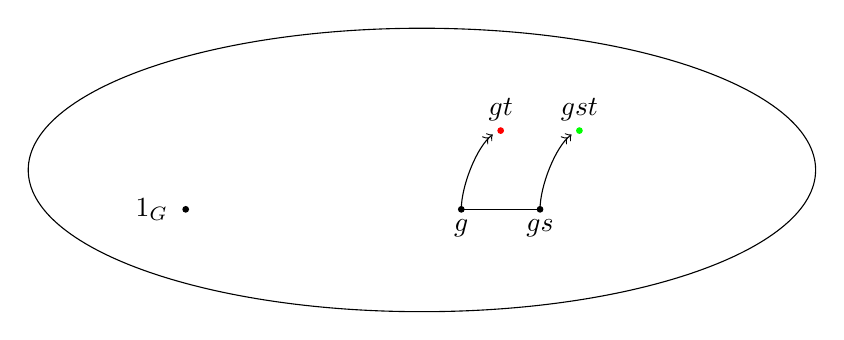
\begin{tikzpicture}

\draw (0,0) ellipse (5 and 1.8);

\filldraw [black]  (-3,-0.5) circle (1pt);

\filldraw [black] (0.5,-0.5) circle (1pt);
\filldraw [black] (1.5,-0.5) circle (1pt);
\filldraw [red] (1.0,0.5) circle (1pt);
\filldraw [green] (2.0,0.5) circle (1pt);


\draw [->>] (0.5,-0.5) .. controls (0.5,-0.2) and (0.7,0.3) .. (0.9,0.45);
\draw [->>] (1.5,-0.5) .. controls (1.5,-0.2) and (1.7,0.3) .. (1.9,0.45);

\draw (-3.1,-0.5) node[anchor=east]  {$1_G$};

\draw (0.5,-0.5) node[anchor=north] {$g$};
\draw (1.5,-0.5) node[anchor=north] {$gs$};
\draw (1.0,0.5) node[anchor=south] {$gt$};
\draw (2.0,0.5) node[anchor=south] {$gst$};
\draw (0.5,-0.5)-- (1.5,-0.5);


\end{tikzpicture}
\end{center}

All the TikZ commands can be used inline using \docAuxCommand{tikz} or within the \docAuxCommand{tikzpicture} environment. When we want to use captions and labels, we enclose it in the figure environment or use \docAuxCommand{captionof}, but it can be called anywhere in the text or math of a Tex document:

\begin{teX}
\begin{figure}
\centering
%\tikzset{external/force remake}
\begin{tikzpicture}
... TikZ commands ...
\end{tikzpicture}
\caption{A diagram drawn with TikZ.}
\label{Fig:_diagram1}
\end{figure}
\end{teX}

We can also use them in math:

\begin{teX}
\begin{align*}
\int dx\; f(x) =
\alpha
%\tikzset{external/force remake}
\begin{tikzpicture}
... TikZ commands ...
\end{tikzpicture}
\end{align*}
\end{teX}



\section{Draw simple lines}

\begin{texexample}{Draw a Line}{ex:line}
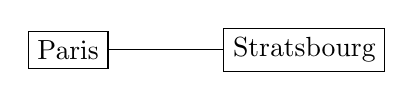
\begin{tikzpicture}
\node[draw] (S1) at (0,0) {Paris};
\node[draw] (S2) at (3,0) {Stratsbourg};
\draw (S1) -- (S2);
\end{tikzpicture}
\end{texexample}


The syntax of the command is:

|\node|\oarg{options} (\meta{name}) at (\meta{position}) |{|\meta{contents}|}|

If we look
 carefully, we see that the two writings give
Slightly different results:
- In the first case, node is an operation executed on a path. We
Can consider each node as a decoration of the point at which it
is associated. The line drawn by the draw command joins two points, the
Nodes are objects added later and centered on points. The option
Draw of the node trace operation the node outline.
- In the second case, \ node is a TikZ command which allows to define
A node, to name it and to draw it. One can then consider the
Nodes as pre-existing objects that will then be linked with the \docAuxCommand{node}.


\begin{texexample}{Draw a Line}{ex:line}
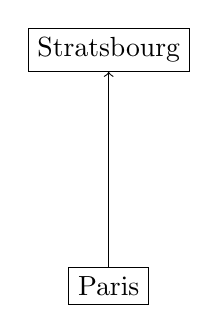
\begin{tikzpicture}
\node[draw] (S1) at (0,0) {Paris};
\node[draw] (S2) at (0,3) {Stratsbourg};
\draw[->] (S1) -- (S2);
\end{tikzpicture}
\end{texexample}

The basic building block of all pictures in \tikzname is the path. A path is a series of straight lines and curves
that are connected (that is not the whole picture, but let us ignore the complications for the moment). You
start a path by specifying the coordinates of the start position as a point in round brackets, as in (0,0).
This is followed by a series of \enquote{path extension operations.}


\begin{texexample}{Draw a Line}{ex:line}
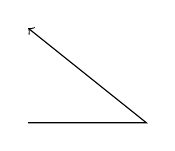
\begin{tikzpicture}
\draw[->] (0,0) -- (1.5,0) -- (0, 1.2);
\end{tikzpicture}
\end{texexample}


\subsection*{Adding Text} 

So far we have seen how to draw lines and arcs. However, an important component is still missing the addition of text. When
\tikzname is constructing a path and it encounters the keyword |node| typically followed by some options  it reads a \textit{node specification}. Options can typically follow and then it terminates by curly brackets. 
 

\begin{texexample}{Draw a Line}{ex:line}
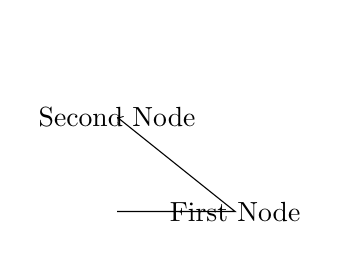
\begin{tikzpicture}
\draw[->] (0,0) -- (1.5,0) node {First Node} -- (0, 1.2) node[shape = circle] {Second Node};
\end{tikzpicture}
\end{texexample}


The \docAuxCommand*{node} can be used to abbreviate the operation. A longer example can demonstrate this better. How can we draw the following figure?

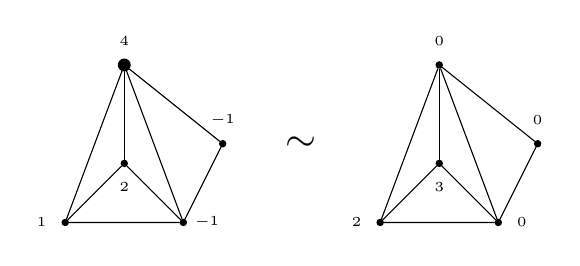
\begin{tikzpicture}
\node[circle,fill=black,inner sep=0.8pt,draw] (a) at (0,0) {};
\node[circle,fill=black,inner sep=0.8pt,draw] (b) at (1.5,0) {};
\node[circle,fill=black,inner sep=1.5pt,draw] (c) at (.75,2) {};
\node[circle,fill=black,inner sep=0.8pt,draw] (d) at (0.75,.75) {};
\node[circle,fill=black,inner sep=0.8pt,draw] (e) at (2,1) {};


\node () at (-0.3,0) {\tiny$1$};
\node () at (0.75,0.45) {\tiny$2$};
\node () at (0.75,2.3) {\tiny$4$};
\node () at (2,1.3) {\tiny$-1$};
\node () at (1.8,0) {\tiny$-1$};

\draw (a)--(b)--(e)--(c) --(a)--(d)--(b)--(c);
\draw (c)--(d);

\node at (3,1) {\Large{$\sim$}};

\begin{scope}[shift={(+4,0)}]
\node[circle,fill=black,inner sep=0.8pt,draw] (a) at (0,0) {};
\node[circle,fill=black,inner sep=0.8pt,draw] (b) at (1.5,0) {};
\node[circle,fill=black,inner sep=0.8pt,draw] (c) at (.75,2) {};
\node[circle,fill=black,inner sep=0.8pt,draw] (d) at (0.75,.75) {};
\node[circle,fill=black,inner sep=0.8pt,draw] (e) at (2,1) {};


\node () at (-0.3,0) {\tiny$2$};
\node () at (0.75,0.45) {\tiny$3$};
\node () at (0.75,2.3) {\tiny$0$};
\node () at (2,1.3) {\tiny$0$};
\node () at (1.8,0) {\tiny$0$};

\draw (a)--(b)--(e)--(c) --(a)--(d)--(b)--(c);
\draw (c)--(d);

\end{scope}
\end{tikzpicture}

\begin{texexample}{A larger example}{ex:larger}
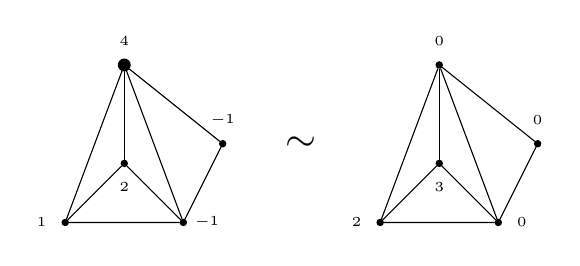
\begin{tikzpicture}
\node[circle,fill=black,inner sep=0.8pt,draw] (a) at (0,0) {};
\node[circle,fill=black,inner sep=0.8pt,draw] (b) at (1.5,0) {};
\node[circle,fill=black,inner sep=1.5pt,draw] (c) at (.75,2) {};
\node[circle,fill=black,inner sep=0.8pt,draw] (d) at (0.75,.75) {};
\node[circle,fill=black,inner sep=0.8pt,draw] (e) at (2,1) {};


\node () at (-0.3,0) {\tiny$1$};
\node () at (0.75,0.45) {\tiny$2$};
\node () at (0.75,2.3) {\tiny$4$};
\node () at (2,1.3) {\tiny$-1$};
\node () at (1.8,0) {\tiny$-1$};

\draw (a)--(b)--(e)--(c) --(a)--(d)--(b)--(c);
\draw (c)--(d);

\node at (3,1) {\Large{$\sim$}};

\begin{scope}[shift={(+4,0)}]
\node[circle,fill=black,inner sep=0.8pt,draw] (a) at (0,0) {};
\node[circle,fill=black,inner sep=0.8pt,draw] (b) at (1.5,0) {};
\node[circle,fill=black,inner sep=0.8pt,draw] (c) at (.75,2) {};
\node[circle,fill=black,inner sep=0.8pt,draw] (d) at (0.75,.75) {};
\node[circle,fill=black,inner sep=0.8pt,draw] (e) at (2,1) {};


\node () at (-0.3,0) {\tiny$2$};
\node () at (0.75,0.45) {\tiny$3$};
\node () at (0.75,2.3) {\tiny$0$};
\node () at (2,1.3) {\tiny$0$};
\node () at (1.8,0) {\tiny$0$};

\draw (a)--(b)--(e)--(c) --(a)--(d)--(b)--(c);
\draw (c)--(d);

\end{scope}
\end{tikzpicture}
\captionof{figure}{The larger vertex fires once to move from the left configuration to the right configuration.}
\end{texexample}

Behind the scenes pgf uses the basic system command \docAuxCommand{pgfnode} to create the nodes. The syntax of the command is given on \seepgfmanual{1026} as:

\begin{docCommand}{pgfnode}{\marg{shape}\marg{anchor}\marg{label text}\marg{name}\marg{path usage command}}
This command creates a new node. The \marg{shape} of the node must have been declared previously using
\lstinline{pgfdeclareshape}.

The shape is shifted such that the \marg{anchor} is at the origin. In order to place the shape somewhere else,
use the coordinate transformation prior to calling this command.
The hnamei is a name for later reference. If no name is given, nothing will be “saved” for the node, it
will just be drawn.

The \marg{path usage command} is executed for the background and the foreground path (if the shape defines
them).
\end{docCommand}


A good workflow, is to first define the nodes, next label them and then draw any connecting lines.

\begin{texexample}{Named nodes}{ex:named} 
\begin{tikzpicture}
\node[circle,fill=black,inner sep=0.8pt,draw] (a) at (0,0) {};
\node[circle,fill=black,inner sep=0.8pt,draw] (b) at (1.5,0) {};
\node[circle,fill=black,inner sep=1.5pt,draw] (c) at (.75,2) {};
\node[circle,fill=black,inner sep=0.8pt,draw] (d) at (0.75,.75) {};
\node[circle,fill=black,inner sep=0.8pt,draw] (e) at (2,1) {};
\end{tikzpicture}
\end{texexample}

\begin{texexample}{Named nodes}{ex:named} 
\begin{tikzpicture}
\node[circle,fill=black,inner sep=0.8pt,draw] (a) at (0,0) {};
\node[circle,fill=black,inner sep=0.8pt,draw] (b) at (1.5,0) {};
\node[circle,fill=black,inner sep=1.5pt,draw] (c) at (.75,2) {};
\node[circle,fill=black,inner sep=0.8pt,draw] (d) at (0.75,.75) {};
\node[circle,fill=black,inner sep=0.8pt,draw] (e) at (2,1) {};
% absolute labelling
\node () at (-0.3,0) {\tiny$1$};
\node () at (0.75,0.45) {\tiny$2$};
\node () at (0.75,2.3) {\tiny$4$};
\node () at (2,1.3) {\tiny$-1$};
\node () at (1.8,0) {\tiny$-1$};
\end{tikzpicture}
\end{texexample}

\begin{texexample}{Named nodes}{ex:named} 
\begin{tikzpicture}
\pgfdeclarelayer{background}
\pgfdeclarelayer{foreground}
\pgfsetlayers{background,main,foreground}
\node[circle,fill=black,inner sep=0.8pt,draw] (a) at (0,0) {};
\node[circle,fill=black,inner sep=0.8pt,draw] (b) at (1.5,0) {};
\node[circle,fill=black,inner sep=1.5pt,draw] (c) at (.75,2) {};
\node[circle,fill=black,inner sep=0.8pt,draw] (d) at (0.75,.75) {};
\node[circle,fill=black,inner sep=0.8pt,draw] (e) at (2,1) {};
% absolute labelling
\node () at (-0.3,0) {\tiny$1$};
\node () at (0.75,0.45) {\tiny$2$};
\node () at (0.75,2.3) {\tiny$4$};
\node () at (2,1.3) {\tiny$-1$};
\node () at (1.8,0) {\tiny$-1$};
% draw connecting lines
\draw (a)--(b)--(e)--(c) --(a)--(d)--(b)--(c);
\draw (c)--(d);
%\begin{pgfonlayer}{background}
\begin{scope}[on background layer={color=blue!10}]
\node [fill=blue!10,fit=(a) (b) (c)
(d) (e)] {};
\end{scope}
%\end{pgfonlayer}
\end{tikzpicture}
\end{texexample}

Just to recap, using \docAuxCommand*{node} and the \textbf{at} we can position accurately any node. We could have used the much longer command |path node|, but in our case above this is unecessary (\seepgfmanual{49}), for more explanations if you are still unsure.

Nodes can be named or unnamed. There are two ways to name them, with the key \docValue{name} or within brackets. The second method is to be preferred. Names for nodes can be pretty arbitrary, but they should not contain commas, periods, parentheses, colons, and some other special characters. However, they can contain underscores and hyphens

\subsection{Layers and Scope}

We can add a backround layer, using the library \textit{backgrounds}, which provides key values for adding backgrounds. \pgfname\ provides a layering mechanism for composing graphics from
multiple layers. (This mechanism is not to be confused with the
conceptual ``software layers'' the \pgfname\ system is composed of.)
Layers are often used in graphic programs. The idea is that you can
draw on the different layers in any order. So you might start drawing
something on the ``background'' layer, then something on the
``foreground'' layer, then something on the ``middle'' layer, and then
something on the background layer once more, and so on. At the end, no
matter in which ordering you drew on the different layers, the layers
are ``stacked on top of each other'' in a fixed ordering to produce
the final picture. Thus, anything drawn on the middle layer would come
on top of everything of the background layer.

Normally, you do not need to use different layers since you will have
little trouble ``ordering'' your graphic commands in such a way that
layers are superfluous. However, in certain situations you only
``know'' what you should draw behind something else after the
``something else'' has been drawn.

For example, suppose you wish to draw a yellow background behind your
picture. The background should be as large as the bounding box of the
picture, plus a little border. If you know the size of the bounding box
of the picture at its beginning, this is easy to accomplish. However,
in general this is not the case and you need to create a
``background'' layer in addition to the standard ``main'' layer. Then,
at the end of the picture, when the bounding box has been established,
you can add a rectangle of the appropriate size to the picture.

\subsection{Declaring Layers}

In \pgfname\ layers are referenced using names. The standard layer,
which is a bit special in certain ways, is called |main|. If nothing
else is specified, all graphic commands are added to the |main|
layer. You can declare a new layer using the following command:

\begin{docCommand}{pgfdeclarelayer}{\marg{name}}
  This command declares a layer named \meta{name} for later
  use. Mainly, this will set up some internal bookkeeping.
\end{docCommand}

The next step toward using a layer is to tell \pgfname\ which layers
will be part of the actual picture and which will be their
ordering. Thus, it is possible to have more layers declared than are
actually used.

\begin{docCommand}{pgfsetlayers}{\marg{layer list}}
  This command tells \pgfname\ which layers will be used in
  pictures. They are stacked on top of each other in the order
  given. The layer |main| should always be part of the list. Here is
  an example:
\begin{codeexample}[code only]
\pgfdeclarelayer{background}
\pgfdeclarelayer{foreground}  
\pgfsetlayers{background,main,foreground}
\end{codeexample}

  This command should be given either outside of any picture or ``directly inside'' of a picture.
  Here, the ``directly inside'' means that there should be no further level of \TeX\ grouping between |\pgfsetlayers| and the matching |\end{pgfpicture}| (no closing braces, no |\end{...}|). It will also work if |\pgfsetlayers| is provided before |\end{tikzpicture}| (with similar restrictions).
\end{docCommand}


\subsection{Using Layers}

Once the layers of your picture have been declared, you can start to
``fill'' them. As said before, all graphics commands are normally
added to the |main| layer. Using the |{pgfonlayer}| environment, you
can tell \pgfname\ that certain commands should, instead, be added to
the given layer.

\begin{docEnvironment}{pgfonlayer}{\marg{layer name}}
\end{docEnvironment}

The whole \meta{environment contents} is added to the layer with the
name \meta{layer name}. This environment can be used anywhere inside
a picture. Thus, even if it is used inside a |{pgfscope}| or a \TeX\
group, the contents will still be added to the ``whole'' picture.
Using this environment multiple times inside the same picture will
cause the \meta{environment contents} to accumulate.

  \emph{Note:} You can \emph{not} add anything to the |main| layer
  using this environment. The only way to add anything to the main
  layer is to give graphic commands outside all |{pgfonlayer}|
  environments. 



\begin{codeexample}[]
\pgfdeclarelayer{background layer}
\pgfdeclarelayer{foreground layer}
\pgfsetlayers{background layer,main,foreground layer}
\begin{tikzpicture}
  % On main layer:
  \fill[blue] (0,0) circle (1cm);
  
  \begin{pgfonlayer}{background layer}
    \fill[yellow] (-1,-1) rectangle (1,1);
  \end{pgfonlayer}
  
  \begin{pgfonlayer}{foreground layer}
    \node[white] {foreground};
  \end{pgfonlayer}
  
  \begin{pgfonlayer}{background layer}
    \fill[black] (-.8,-.8) rectangle (.8,.8);
  \end{pgfonlayer}

  % On main layer again:
  \fill[blue!50] (-.5,-1) rectangle (.5,1);
\end{tikzpicture}
\end{codeexample}



\long\gdef\mytriangle{
\node[circle,fill=black,inner sep=0.8pt,draw] (a) at (0,0) {};
\node[circle,fill=black,inner sep=0.8pt,draw] (b) at (1.5,0) {};
\node[circle,fill=black,inner sep=1.5pt,draw] (c) at (.75,2) {};
\node[circle,fill=black,inner sep=0.8pt,draw] (d) at (0.75,.75) {};
\node[circle,fill=black,inner sep=0.8pt,draw] (e) at (2,1) {};
% absolute labelling
\node () at (-0.3,0) {\tiny$1$};
\node () at (0.75,0.45) {\tiny$2$};
\node () at (0.75,2.3) {\tiny$4$};
\node () at (2,1.3) {\tiny$-1$};
\node () at (1.8,0) {\tiny$-1$};
% draw connecting lines
\draw (a)--(b)--(e)--(c) --(a)--(d)--(b)--(c);
\draw (c)--(d);
}

\begin{texexample}{Adding backgrouns}{ex:backgrounds}
\begin{tikzpicture}
\pgfdeclarelayer{background}
\pgfdeclarelayer{foreground}
\pgfsetlayers{background,main,foreground}
\mytriangle
%\begin{pgfonlayer}{background}
\begin{scope}[on background layer={color=blue!10}]
\mytriangle
\node [fill=blue!10,fit=(a) (b) (c)
(d) (e)] {};
\end{scope}
%\end{pgfonlayer}
\end{tikzpicture}
\end{texexample}


\begin{texexample}{Adding backgrouns}{ex:backgrounds}
\begin{tikzpicture}
\pgfdeclarelayer{background}
\pgfdeclarelayer{foreground}
\pgfsetlayers{background,main,foreground}
\mytriangle
%\begin{pgfonlayer}{background}
\begin{scope}[on background layer={color=blue!10}]
\node [fill=blue!10,fit=(a) (b) (c)
(d) (e)] {};
\end{scope}

\begin{scope}[shift={(+4,0)}]
\mytriangle
\begin{pgfonlayer}{background}
\node [pattern=checkerboard light gray,fit=(a) (b) (c)
(d) (e)] {};
\end{pgfonlayer}
\end{scope}
\end{tikzpicture}
\end{texexample}

This brings us to the end of our discussion. Time for a coffee and a break.                

\section{Adding styles}

In our previous example, we cut and pasted many of the repetitive keys. \pgfname offers a way to set a new key to the values of other keys using the handler |.style|. This is a very powerful way of redefining new keys, but also simplifying the code. Styles in \tikzname can be considered similar to macros in standard LaTeX. When I made a drawing, we can still tweak the styles and look how the drawing changes, until it's perfect. You should never have to tweak each node.

\begin{texexample}{Using styles}{ex:usingstyles}
\tikzset{BN/.style = {circle,fill=black,inner sep=0.8pt,draw},
         tiny/.style = {font=\tiny}, 
}
\begin{tikzpicture}
\node[BN] (a) at (0,0) {};
\node[BN] (b) at (1,0) {};
\node[BN] (c) at (1,1) {};
\node[BN] (d) at (0,1) {};
\node[BN] (e) at (-1,0) {};

\node () at (-1.3,0) [tiny]{$v_1$};
\node () at (-.3,1)  [tiny]{$v_2$};
\node () at (1.3,0)  [tiny]{$w_1$};
\node () at (1.3,1)  [tiny]{$w_2$};

\node[tiny] () at (0.5,-0.2) {$a$};
\node[tiny] () at (0.5,1.2) {$b$};
\node[tiny] () at (0.2,0.5) {$c$};
\node[tiny] () at (-0.5,-.2) {$d$};

\draw (e) -- (a) -- (b) -- (c) -- (d) -- (a);
\draw (e) -- (d);

\end{tikzpicture}
\end{texexample}



\section{Arcs and options for lines}

\begin{texexample}{Draw a Line}{ex:line}
\begin{tikzpicture}
\draw[->] (0,0) -- (1.5,0) node[draw, ellipse] {First Node} -| (0, 1.2) node[draw,ellipse,rotate=45] {Second Node};
\end{tikzpicture}
\end{texexample}

\begin{texexample}{Drawing arcs}{ex:matharcs}
We define 
\begin{gather*}
    \bar{d}_{k,l}:=\hspace{6pt}
    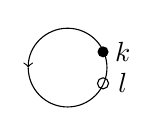
\begin{tikzpicture}[baseline=(current bounding box.center)]
    \draw[->] (3,2) arc (-180:180:5mm);
	  \fill (3.95,2.2) circle [radius=2pt];
    \draw (3.95,1.8) circle [radius=2pt];
    \node at (4.2,1.8) {$l$};
    \node at (4.2,2.2) {$k$};
    \end{tikzpicture}
    \hspace{0.5cm}
    \text{and}
    \hspace{0.5cm}
    d_{k,l}:=\hspace{6pt}
    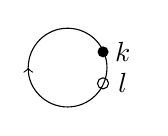
\begin{tikzpicture}[baseline=(current bounding box.center)]
    \draw[<-] (3,2) arc (-180:180:5mm);
    \fill (3.95,2.2) circle [radius=2pt];
    \draw (3.95,1.8) circle [radius=2pt];
    \node at (4.2,1.8) {$l$};
    \node at (4.2,2.2) {$k$};
    \end{tikzpicture}
    \hspace{0.5cm}
    \text{for}
    \hspace{2mm} k,l\in\mathbb{Z}_{\geq 0}.
\end{gather*}
\end{texexample}


Here is a figure that you should try and reproduce.
\newcommand{\G}{\Gamma}

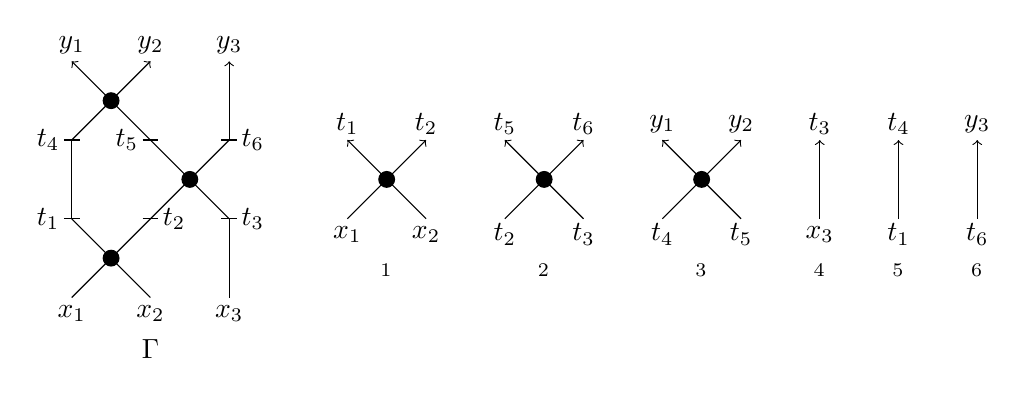
\begin{tikzpicture}
\draw (-3.5,-1)--(-2.5,0); \draw (-2.5,-1)--(-3.5,0); \draw (-1.5,-1)--(-1.5,0);\draw[fill=black] (-3,-0.5) circle (0.1cm); \draw (-3.5,0)--(-3.5,1); \draw (-2.5,0)--(-1.5,1); \draw (-1.5,0)--(-2.5,1);\draw[fill=black] (-2,0.5) circle (0.1cm); \draw[->] (-3.5,1)--(-2.5,2); \draw[->] (-2.5,1)--(-3.5,2); \draw[->] (-1.5,1)--(-1.5,2); \draw[fill=black] (-3,1.5) circle (0.1cm); \draw (-3.6,0)--(-3.4,0);\draw (-2.6,0)--(-2.4,0);\draw (-1.6,0)--(-1.4,0); \draw (-3.6,1)--(-3.4,1);\draw (-2.6,1)--(-2.4,1);\draw (-1.6,1)--(-1.4,1); \node at (-3.5,-1.2) {$x_1$};\node at (-2.5,-1.2) {$x_2$};\node at (-1.5,-1.2) {$x_3$}; \node at (-3.5,2.2) {$y_1$};\node at (-2.5,2.2) {$y_2$};\node at (-1.5,2.2) {$y_3$}; \node at (-3.8,0) {$t_1$};\node at (-2.2,0) {$t_2$};\node at (-1.2,0) {$t_3$}; \node at (-3.8,1) {$t_4$};\node at (-2.8,1) {$t_5$};\node at (-1.2,1) {$t_6$}; \node at (-2.5,-1.65) {$\Gamma$};
\draw[->] (0,0)--(1,1); \draw[->] (1,0)--(0,1); \draw[fill=black] (0.5,0.5) circle (0.1cm); \draw[->] (2,0)--(3,1); \draw[->] (3,0)--(2,1); \draw[fill=black] (2.5,0.5) circle (0.1cm); \draw[->] (4,0)--(5,1); \draw[->] (5,0)--(4,1); \draw[fill=black] (4.5,0.5) circle (0.1cm); \draw[->] (6,0)--(6,1); \draw[->] (7,0)--(7,1); \draw[->] (8,0)--(8,1);
\node at (0,-.2) {$x_1$};\node at (1,-.2) {$x_2$}; \node at (2,-.2) {$t_2$};\node at (3,-.2) {$t_3$}; \node at (4,-.2) {$t_4$};\node at (5,-.2) {$t_5$}; \node at (6,-.2) {$x_3$}; \node at (7,-.2) {$t_1$}; \node at (8,-.2) {$t_6$};
\node at (0,1.2) {$t_1$};\node at (1,1.2) {$t_2$}; \node at (2,1.2) {$t_5$};\node at (3,1.2) {$t_6$}; \node at (4,1.2) {$y_1$};\node at (5,1.2) {$y_2$}; \node at (6,1.2) {$t_3$}; \node at (7,1.2) {$t_4$}; \node at (8,1.2) {$y_3$};
\node at (0.5,-0.65) {$\G_1$}; \node at (2.5,-0.65) {$\G_2$}; \node at (4.5,-0.65) {$\G_3$}; \node at (6,-0.65) {$\G_4$};\node at (7,-0.65) {$\G_5$};\node at (8,-0.65) {$\G_6$}; 
\end{tikzpicture}

This brings us to the end.




The |node| can take numerous options who are then used to set the typesetting of the text that follows:


\begin{texexample}{Draw a Line}{ex:line}
\begin{tikzpicture}
\draw[->] (0,0) -- (1.5,0) node[draw, ellipse] {First Node} -| (0, 1.2) node[draw,ellipse,rotate=45, text width=3cm, fill=creamy, text justified] {\lorem};
\end{tikzpicture}
\end{texexample}


\begin{texexample}{Draw a Line}{ex:line}
\begin{tikzpicture}[funny ellipse/.style = {draw,ellipse,rotate=45, text width=3cm, fill=creamy, text justified} ]
\draw[->] (0,0) -- (1.5,0) node[draw, ellipse] {First Node} -| (0, 1.2) node[funny ellipse] {\lorem};
\end{tikzpicture}
\end{texexample}

This can also be written by using \docAuxCommand{tikzset} for setting out all the keys. This can written just before the environment or within the scope of the environment. See \href{https://tex.stackexchange.com/questions/52372/should-tikzset-or-tikzstyle-be-used-to-define-tikz-styles}{TX.SX discussion}, for the option to set |\tikzstyle| which should not be used, even if it is quicker to write.


\begin{texexample}{Draw a Line}{ex:line}
\tikzset{funny ellipse/.style = {draw,ellipse,rotate=45, text width=3cm, fill=creamy, text justified} }
\begin{tikzpicture}
\draw[->] (0,0) -- (1.5,0) node[draw, ellipse] {First Node} -| (0, 1.2) node[funny ellipse] {\lorem};
\end{tikzpicture}
\end{texexample}

A |node| can possibly be rendered with a choice from a list of over 720 keys.

ed. 



Using the |TikZ| package you can draw figures and intermingle them with text. To draw a simple diamond as shown in \fref{fig:diamond} we use
the following commands. The package comes with a very comprehensive manual of over 500 pages long. One can state that there is nothing that you cannot draw with PGF/TikZ, if you have the patience and perseverance. TikZ's language has a syntax of its own with very little connection to what we have used so far. You will need to set aside adequate time to study this, especially if your work has a lot of specially drawn figures that you need. The result like anything else in \tex make the effort worthwhile.

\begin{texexample}{Draw a Diamond}{fig:diamond}

\begin{tikzpicture}
 \draw (1,0) -- (0,1) -- (-1,0) -- (0,-1) -- cycle;
\end{tikzpicture}
\end{texexample}


\begin{texexample}{Text long path}{ex:decorations}
\begin{tikzpicture}
\draw [help lines] grid (3,2);
\draw [red, dashed]
[postaction={decoration={text along path, text={a big juicy apple},
text align=fit to path}, decorate}]
(0,0) .. controls (0,2) and (3,2) .. (3,0);
\node (A) at (1.5,0) {!};
\end{tikzpicture}
\end{texexample}


\begin{texexample}{Text long path}{ex:decorations}

Hello \begin{pgfpicture}
\pgfpathrectangle{\pgfpointorigin}{\pgfpoint{2ex}{1ex}}
\pgfusepath{stroke}
\end{pgfpicture} World!

\end{texexample}


\emphasis{-,draw,begin,end,tikzpicture}
\begin{teXXX}

\begin{tikzpicture}
\draw (1,0) -- (0,1) -- (-1,0) -- (0,-1) -- cycle;
\end{tikzpicture}
\end{teXXX}



\makeatletter
The value of $x$ is \pgfsys@markposition{here}important.

Lots of text.
\hbox{\pgfsys@markposition{myorigin}%
\begin{pgfpicture}
% Switch of size protocol
\pgfpathmoveto{\pgfpointorigin}
\pgfusepath{use as bounding box}
\pgfsys@getposition{here}{\hereposition}
\pgfsys@getposition{myorigin}{\thispictureposition}
\pgftransformshift{\pgfpointscale{-1}{\thispictureposition}}
\pgftransformshift{\hereposition}
\pgfpathcircle{\pgfpointorigin}{1cm}
\pgfusepath{draw}
\end{pgfpicture}}

\makeatother


You cannot write directly into a picture environment. The command \docAuxCommand{pgftext} can be used. 

\begin{texexample}{Using text directly}{ex:pgftext}
\tikz{\draw[help lines] (0,0) grid (3,2);
\pgftext[base,x=1cm,y=0.5cm] {lovely}}
\end{texexample}





Sometimes it is quite useful when debugging to add a backround grid. 


\begin{centering}
\begin{tikzpicture}
\draw[step=0.25cm,color=creamy] (-1,-1) grid (1,1);
\draw [color=bgsexy](1,0) -- (0,1) -- (-1,0) -- (0,-1) -- cycle;
\end{tikzpicture}
\captionof{figure}{You can add a background grid using \texttt{step=0.25cm, color=green} as an option}
\end{centering}


\emphasis{step,color,green,grid,begin,end}
\begin{teXXX}
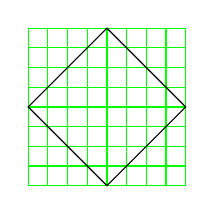
\begin{tikzpicture}
  \draw[step=0.25cm,color=green] (-1,-1) grid (1,1);
  \draw (1,0) -- (0,1) -- (-1,0) -- (0,-1) -- cycle;
\end{tikzpicture}
\end{teXXX}

The grid is specified by providing two diagonally opposing points: (-1,-1)
and (1, 1). The two options supplied give a step size for the grid lines and a
specification for the color of the grid lines, using the \docpkg{xcolor} package

\subsection{Specifying points and paths}

\begin{texexample}{Specifying points and paths}{ex:points}
\centering
\begin{tikzpicture}[scale=1.8]
% Define the points of a regular pentagon
\path (0,0) coordinate (origin);
\path (0:1cm) coordinate (P0);
\path (1*72:1cm) coordinate (P1);
\path (2*72:1cm) coordinate (P2);
\path (3*72:1cm) coordinate (P3);
\path (4*72:1cm) coordinate (P4);
% Draw the edges of the pentagon
\draw[color=bgsexy] (P0) -- (P1) -- (P2) -- (P3) -- (P4) -- cycle;
% Add "spokes"
\draw[color=red800] (origin) -- (P0) (origin) -- (P1) (origin) -- (P2)
(origin) -- (P3) (origin) -- (P4);
\end{tikzpicture}
\captionof{figure}{Drawing a complicated polygon, using paths and the \texttt{draw} command}
\end{texexample}


Two key ideas used in \tikzname\ are points and paths. Both of these ideas were used
in the diamond examples. Much more is possible, however. For example, points
can be specified in any of the following ways:
\begin{enumerate}
\item  Cartesian coordinates
\item  Polar coordinates
\item  Named points
\item  Relative points
\end{enumerate}



\subsection{coordinates}
The cartesian coordinates can be defined and named using the following syntax.

%\emphasis{begin,end,coordinate,at,draw}
%\begin{teXXX}
%\begin{tikzpicture}
%  \coordinate (A) at (0,0);
%  \coordinate (B) at (1.25,0.25);
%  \draw[blue] (A) -- (B);
%\end{tikzpicture}
%\end{teXXX}

\noindent This produces:
\begin{tikzpicture}
\coordinate (A) at (0,0);
\coordinate (B) at (1.25,0.25);
\draw[blue] (A) -- (B);
\end{tikzpicture}


We can add labels to the points by using the |label| option. A label is distinct from the text of a |node|.

\begin{tikzpicture}
\coordinate [label=left:\textcolor{orange}{$A$}] (A) at (0,0);
\coordinate [label=right:\textcolor{orange}{$B$}]  (B) at (1.15,0.25);
\draw[blue] (A) -- (B);
\end{tikzpicture}

\emphasis{label,left,label:,right}
\begin{teXXX}
\begin{tikzpicture}
  \coordinate [label=left:\textcolor{orange}{$A$}] (A) at (0,0);
  \coordinate [label=west:\textcolor{orange}{$B$}] (B) at (1.25,0.25);
  \draw[blue] (A) -- (B);
\end{tikzpicture}
\end{teXXX}




If you tempted to write \texttt{label=top:} it will not work, as the command accepts the following keywords.


\begin{tikzpicture}
  \coordinate [label=left:\textcolor{orange}{east}]  (A) at (0,0);
  \coordinate [label=right:\textcolor{orange}{west}] (B) at (0,0);
  \draw[blue] (A)--(B);
\end{tikzpicture}


\section{Graphic Parameters: Line Width, Line Cap, and Line Join}

The width of lines can be specified using the key:

\begin{docKey}[tikz]{line width}{=\marg{dimension}} {no default, initially 0.4pt}
Specifies the line width \seepgfmanual{166}
\end{docKey}



\bgroup
\def\mkl#1{\tikz \draw[#1] (0,0)--(1.0, 1.5ex);}
\scriptsize\arial
\begin{tabular}{|l|l|l|l|l|l|l|l|}
\hline
\mkl{line width=2pt}& \mkl{ultra thin} &\mkl{very thin} & \mkl{thin} & \mkl{semithick} & \mkl{thick} &\mkl{very thick} &\mkl{ultra thick} \\
\hline
line width=2pt &ultra thin & very thin & thin &semithick & thick & very thick & ultra thick \\
\hline
\end{tabular}
\egroup

\begin{docKey}[tikz]{line cap}{=\marg{dimension}} {no default, initially 0.4pt}
Specifies how lines “end.” Permissible types are round, rect, and butt \seepgfmanual{167}. 
\end{docKey}

\bgroup
\def\mkl#1{\begin{tikzpicture} \draw[line width=10pt, line cap=#1] (0,0)--(1.0, 1.5ex);\draw[white,line width=2pt]
(0,0 )--(1.0,1.5ex);\end{tikzpicture}}
\scriptsize\arial
\begin{tabular}{|l|l|l|}
\hline
\mkl{rect}& \mkl{butt} &\mkl{round}  \\
\hline
rect &butt & round \\
\hline
\end{tabular}
\egroup




\begin{docKey}[tikz]{line join}{=\marg{type}}{no default, initially miter}
Specifies how lines “join.” Permissible type are round, bevel, and miter. They have the following
effects:
\end{docKey}

\begin{texexample}{Joining Lines}{es:joinlines}

\begin{tikzpicture}[line width=10pt]
\draw[line join=round] (0,0) -- ++(.5,1) -- ++(.5,-1);
\draw[line join=bevel] (1.25,0) -- ++(.5,1) -- ++(.5,-1);
\draw[line join=miter] (2.5,0) -- ++(.5,1) -- ++(.5,-1);
\end{tikzpicture}
\end{texexample}


\begin{docKey}[tikz]{dash pattern}{=\marg{dash pattern}}{no default}
Sets the dashing pattern. The syntax is the same as in \metafontlogo. For example following pattern on
2pt off 3pt on 4pt off 4pt means \enquote{draw 2pt, then leave out 3pt, then draw 4pt once more, then
leave out 4pt again, repeat}.
\end{docKey}

\bgroup
\def\ml#1{\tikz \draw[ #1] (0pt,0pt) -- (50pt,0pt);}
\def\alist{solid, dotted, densely dotted, loosely dotted,% 
           dashed,densely dashed, loosely dashed, %
           dash dot, densely dash dot, loosely dash dot, %
           dash dot dot, densely dash dot dot, loosely dash dot dot.}

For patterns there are numerous settings {\arial \alist }


\scriptsize
\begin{tabular}{lll}
\hline
\ml{solid} &  & \\
solid      &  & \\
\hline
\ml{dotted} &\ml{densely dotted} & \ml{loosely dotted}\\
\textit{dotted} & densely dotted  &loosely dotted \\
\hline
\ml{dashed} & \ml{densely dashed} & \ml{loosely dashed}  \\
\textit{dashed}      & densely dashed & loosely dashed            \\
\hline

\ml{dash dot} & \ml{densely dash dot} & \ml{loosely dash dot} \\
\textit{dash dot} & densely dash dot & loosely dash dot \\
\hline

\ml{dash dot dot} & \ml{densely dash dot dot} & \ml{loosely dash dot dot} \\
\textit{dash dot dot} & densely dash dot dot & loosely dash dot dot \\
\hline
\end{tabular}
\egroup


\subsection{Pattern Library}

The library patterns can be used to draw predetermined patterns. This will be a longer than usual section as it explains how to create new patterns. Most of the content is straight from the \pgfname manual. Before we start with the creation f a new pattern let us examine how a pattern is used.

\begin{texexample}{Using Library Patterns}{ex:libpatterns}
\begin{tikzpicture}
\pattern [path fading=west,pattern=checkerboard light gray]
      (0,0) rectangle (5cm,2em);
\end{tikzpicture}
\end{texexample}


\label{section-library-patterns}


The package defines patterns for filling areas. \docAuxCommand*{usetikzlibrary}\marg{patterns}.




\subsection{Form-Only Patterns}

\begin{tabular}{ll}
  \emph{Pattern name} & \emph{Example (pattern in black, blue, and red
    on faded checkerboard)} \\ 
  \patternindex{horizontal lines} 
  \patternindex{vertical lines} 
  \patternindex{north east lines} 
  \patternindex{north west lines} 
  \patternindex{grid} 
  \patternindex{crosshatch} 
  \patternindex{dots} 
  \patternindex{crosshatch dots} 
  \patternindex{fivepointed stars} 
  \patternindex{sixpointed stars} 
  \patternindex{bricks}
  \patternindex{checkerboard}
\end{tabular}
  
\subsection{Inherently Colored Patterns}


\begin{tabular}{ll}
  \emph{Pattern name} & \emph{Example} \\
  \patternindexinherentlycolored{checkerboard light gray} 
  \patternindexinherentlycolored{horizontal lines light gray} 
  \patternindexinherentlycolored{horizontal lines gray} 
  \patternindexinherentlycolored{horizontal lines dark gray} 
  \patternindexinherentlycolored{horizontal lines light blue} 
  \patternindexinherentlycolored{horizontal lines dark blue} 
  \patternindexinherentlycolored{crosshatch dots gray} 
  \patternindexinherentlycolored{crosshatch dots light steel blue} 
\end{tabular}
  


% Copyright 2006 by Till Tantau
%
% This file may be distributed and/or modified
%
% 1. under the LaTeX Project Public License and/or
% 2. under the GNU Free Documentation License.
%
% See the file doc/generic/pgf/licenses/LICENSE for more details.


\section{Creating Patterns}

\label{section-patterns}

\subsection{Overview}

There are many ways of filling a path. First, you can fill it using a
solid color and this is also the fastest method. Second, you can also
fill it using a shading, which means that the color changes smoothly
between two (or more) different colors. Third, you can fill it using a
tiling pattern and it is explained in the following how this is done.

A tiling pattern can be imagined as a rectangular tile (hence the
name) on which a small picture is painted. There is not a single tile,
but (conceptually) an infinite number of tiles, all showing the same
picture, and these tiles are arranged horizontally and vertically to
fill the plane. When you use a tiling pattern to fill a path, what
happens is that the path clips out a ``window'' through which we see
part of this infinite plane.

Patterns come in two versions: \emph{inherently colored patterns} and
\emph{form-only patterns}. (These are often called ``color patterns''
and ``uncolored patterns,'' but these names are misleading since
uncolored patterns do have a color and the color changes. As I said,
the name is misleading\dots) An inherently colored pattern is just a
colored tile like, say, a red star with a black outline. A form-only
pattern can be imagined as a tile that is a kind of rubber stamp. When
this pattern is used, the stamp is used to print copies of the stamp
picture onto the plane, but we can use a different stamp color each
time we use a form-only pattern.

\pgfname\ provides a special support for patterns. You can declare a
pattern and then use it very much like a fill color. \pgfname\
directly maps patterns to the pattern facilities of the underlying
graphic languages (PostScript, \textsc{pdf}, and \textsc{svg}). This
means that filling a path using a pattern will be nearly as fast as if
you used a uniform color.

There are a number of pitfalls and restrictions when using
patterns. First, once a pattern has been declared, you cannot change
it anymore. In particular, it is not possible to enlarge it or change
the line width. Such flexibility would require that the repeating of
the pattern were not done by the graphic language, but on the
\pgfname\ level. This would make patterns orders of magnitude slower
to produce and to render. However, \pgfname{} does provide a
more-or-less successful emulation of ``mutable'' patterns, although
internally, a new (fixed) instance of a pattern is declared when
the parameters of a pattern change.

Second, the phase of patterns is not well-defined, that is, it is not
clear where the origin of the ``first'' tile is. To be more precise,
PostScript and \textsc{pdf} on the one hand and \textsc{svg} on the
other hand define the origin differently. PostScript and \textsc{pdf}
define a fixed origin that is independent of where the path lies. This
has the highly desirable effect that if you use the same pattern to
fill multiple paths, the outcome is the same as if you had filled a 
single path consisting of the union of all these paths. By
comparison, \textsc{svg} uses the upper-left (?) corner of the path to
be filled as the origin. However, the \textsc{svg} specification is a
bit vague on this question.


\subsection{Declaring a Pattern}

Before a pattern can be used, it must be declared. The following
command is used for this:

\begin{docCommand}{pgfdeclarepatternformonly}{%
	\oarg{variables}%
	\marg{name}%
	\marg{bottom left}%
	\marg{top right}%
	\marg{tile size}%
	\marg{code}}

	This command declares a new form-only pattern. The \meta{name} is a
  name for later reference. The two parameters \meta{lower left} and
  \meta{upper right} must describe a bounding box that is large enough
  to encompass the complete tile.
\end{docCommand}

  The size of a tile is given by \meta{tile size}, that is, a tile is
  a rectangle whose lower left   corner is the origin and whose upper
  right corner is given by \meta{tile size}. This might make you
  wonder why the second and third parameters are needed. First, the
  bounding box might be smaller than the tile size if the tile is
  larger than the picture on the tile. Second, the bounding box might
  be bigger, in which case the picture will ``bleed'' over the tile.

  The \meta{code} should be \pgfname\ code than can be protocolled. It
  should not contain any color code.


\begin{codeexample}[]
\pgfdeclarepatternformonly{stars}
{\pgfpointorigin}{\pgfpoint{1cm}{1cm}}
{\pgfpoint{1cm}{1cm}}
{
  \pgftransformshift{\pgfpoint{.5cm}{.5cm}}
  \pgfpathmoveto{\pgfpointpolar{0}{4mm}}
  \pgfpathlineto{\pgfpointpolar{144}{4mm}}
  \pgfpathlineto{\pgfpointpolar{288}{4mm}}
  \pgfpathlineto{\pgfpointpolar{72}{4mm}}
  \pgfpathlineto{\pgfpointpolar{216}{4mm}}
  \pgfpathclose%
  \pgfusepath{fill}
}
\begin{tikzpicture}
  \filldraw[pattern=stars] (0,0)   rectangle (1.5,2);
  \filldraw[pattern=stars,pattern color=red]
                           (1.5,0) rectangle (3,2);
\end{tikzpicture}
\end{codeexample}

	The optional argument \meta{variables} consists of a comma
	separated	list of macros,	registers or keys, representing the
	parameters of the pattern that may vary. If a variable is a key,
	then the full path name must be used (specifically, it must start
	with |/|).
	As an example, a list might look like the following:
	|\mymacro,\mydimen,/pgf/my key|. Note that macros and keys should
	be ``simple''. They should only store values in themselves.
	
	The effect of \meta{variables}, is the following:
  Normally, when this argument is empty, once a pattern has been
  declared, it becomes ``frozen''. This means that it is not possible
  to enlarge the pattern or change the line width later on.
  By specifying \meta{variables}, no pattern is actually created.
  Instead, the arguments are stored away
  (so the macros,	registers or keys do not have to be defined in advance).

  When the fill pattern is set, \pgfname{} checks if the pattern has
  already been created with the \meta{variables} set to their current
  values (\pgfname{} is usually ``smart enough'' to distinguish between
  macros, registers and keys). If so, this already-declared-pattern
  is used as the fill pattern.
  If not, a new instance of the pattern (which will have a
  unique internal name) is declared using the current values of
  \meta{variables}. These values are then saved and the fill pattern
  set accordingly.
	
	The following shows an example of a pattern which varies
	according to the values of the macro |\size|, the key |/tikz/radius|,
	and the \TeX{} dimension |\thickness|.

\begin{texexample}{New Pattern Example}{ex:newpattern}
\pgfdeclarepatternformonly[/tikz/radius,\thickness,\size]{rings}
{\pgfpoint{-0.5*\size}{-0.5*\size}}
{\pgfpoint{0.5*\size}{0.5*\size}}
{\pgfpoint{\size}{\size}}
{
  \pgfsetlinewidth{\thickness}
  \pgfpathcircle\pgfpointorigin{\pgfkeysvalueof{/tikz/radius}}
  \pgfusepath{stroke}
}
\newdimen\thickness
\tikzset{
  radius/.initial=4pt,
  size/.store in=\size, size=20pt,
  thickness/.code={\thickness=#1},
  thickness=0.75pt
}
\begin{tikzpicture}[rings/.style={pattern=rings}]
  \filldraw [rings, radius=2pt, size=6pt]      (0,0)   rectangle +(1.5,2);
  \filldraw [rings, radius=2pt, size=8pt]      (2,0)   rectangle +(1.5,2);
  \filldraw [rings, radius=6pt, thickness=2pt] (0,2.5) rectangle +(1.5,2);
  \filldraw [rings, radius=8pt, thickness=4pt] (2,2.5) rectangle +(1.5,2);
\end{tikzpicture}
\end{texexample}



\begin{docCommand}{pgfdeclarepatterninherentlycolored}{\oarg{variables}
    \marg{name}
    \marg{lower left}
    \marg{upper right}
    \marg{tile size}
    \marg{code}}
  This command works like |\pgfdeclarepatternuncolored|, only the
  pattern will have an inherent color. To set the color, you should
  use \pgfname's color commands, not the |\color| command, since this
  fill is not protocolled.
\end{docCommand}

\begin{texexample}{Inherently Colored}{ex:ingerentlycolored}
\pgfdeclarepatterninherentlycolored{green stars}
{\pgfpointorigin}{\pgfpoint{1cm}{1cm}}
{\pgfpoint{1cm}{1cm}}
{
  \pgfsetfillcolor{green!50!black}
  \pgftransformshift{\pgfpoint{.5cm}{.5cm}}
  \pgfpathmoveto{\pgfpointpolar{0}{4mm}}
  \pgfpathlineto{\pgfpointpolar{144}{4mm}}
  \pgfpathlineto{\pgfpointpolar{288}{4mm}}
  \pgfpathlineto{\pgfpointpolar{72}{4mm}}
  \pgfpathlineto{\pgfpointpolar{216}{4mm}}
  \pgfpathclose%
  \pgfusepath{stroke,fill}
}
\begin{tikzpicture}
  \filldraw[pattern=green stars] (0,0) rectangle (3,2);
\end{tikzpicture}
\end{texexample}



\subsection{Setting a Pattern}

Once a pattern has been declared, it can be used.

\begin{docCommand}{pgfsetfillpattern}{\marg{name}\marg{color}}
  This command specifies that paths that are filled should be filled
  with the ``color'' by the pattern \meta{name}. For an inherently
  colored pattern, the \meta{color} parameter is ignored. For
  form-only patterns, the \meta{color} parameter specifies the color
  to be used for the pattern.
\end{docCommand}
  
\begin{codeexample}[]
\begin{tikzpicture}
  \pgfsetfillpattern{stars}{red}
  \filldraw (0,0) rectangle (1.5,2);

  \pgfsetfillpattern{green stars}{red}
  \filldraw (1.5,0) rectangle (3,2);
\end{tikzpicture}
\end{codeexample}



\endinput
%To summarize, what we have been doing so far is to learn a set of primitive TikZ commands for drawing paths, drawing shapes and labeling them. All TikZ command work by passing options to them. For example to change the above line to an arrow, we just pass the option |->| to the |draw| command.
%

%\begin{tikzpicture}
%  \coordinate [label=left:\textcolor{orange}{$A$}] (A) at (0,0);
%  \coordinate [label=right:\textcolor{orange}{$B$}] (B) at (1.25,0.25);
%  \draw[->,o-stealth] (A)--(B);
%\end{tikzpicture}
%\caption{Effect of the option \protect\texttt{draw[->]}.}

%\emphasis{begin,end,->,draw}
%\begin{teXXX}
%\begin{tikzpicture}
%  ...
%  ...
%  \draw[->,blue] (A)--(B);
%\end{tikzpicture}
%\end{teXXX}
%
%\section*{Relative coordinates}
%\index{TikZ!coordinates, relative}
%A coordinate can be made "relative" by prefixing it with |++|. relative coordinates are useful in many applications.
%\medskip
%
%\noindent The code is simple, except before the coordinate you add the |++| signs. This tells the PGF engine to add the x,y dimensions of the new coordinate to that of its predecessor's. In many instances this is more intuitive and easier to determine.



%\begin{tikzpicture}
%\draw[step=0.5cm,color=gray] (-1,-1) grid (3.5,3);
%\draw[->,red,thick] (0,0) -- ++(1,0) -- ++(0,1) -- ++(-1,0) -- cycle;
%\draw[->,red,thick] (2,0) -- ++(1,0) -- ++(0,1) -- ++(-1,0) -- cycle;
%\draw[arrows=o-stealth,blue] (1.5,1.5) -- ++(1,0) -- ++(0,1) -- ++(-1,0) -- cycle;
%\end{tikzpicture}
%\caption{Example of use of the \protect\texttt{++} to specify relative coordinates.}
%\label{fig:relative}

%\begin{teXXX}
%\begin{tikzpicture}
%  \draw[step=0.5cm,color=gray] (-1,-1) grid (3.5,3);
%  \draw[red,very thick] (0,0) -- ++(1,0) -- ++(0,1) -- ++(-1,0) -- cycle;
%  \draw[red,very thick] (2,0) -- ++(1,0) -- ++(0,1) -- ++(-1,0) -- cycle;
%  \draw[->,red,very thick] (1.5,1.5) -- ++(1,0) -- ++(0,1) -- ++(-1,0) -- cycle;
%\end{tikzpicture}
%\end{teXXX}
%
%Instead of |++| you can also use a single |+|. This also specifies a relative coordinate, but it does not "update"
%the current point for subsequent usages of relative coordinates. Thus, you can use this notation to specify
%numerous points, all relative to the same "initial" point:
%

%\begin{tikzpicture}
%\draw[step=0.5cm,color=gray] (-1,-1) grid (3.5,3);
%\draw[purple, fill=white] (0,0) -- +(1,0) -- +(1,1) -- +(0,1) -- cycle;
%\draw[purple, fill=white] (2,0) -- +(1,0) -- +(1,1) -- +(0,1) -- cycle;
%\draw[purple, fill=white] (1.5,1.5) -- +(1,0) -- +(1,1) -- +(0,1) -- cycle;
%\path (0,0) node [shape=circle,draw]{(0,0)};
%\end{tikzpicture}
%\caption{Example of use of the \protect\texttt{+} to specify relative coordinates.}
%\label{fig:relative1}

%\begin{teXXX}
%  \draw (0,0) -- +(1,0) -- +(1,1) -- +(0,1) -- cycle;
%  \draw (2,0) -- +(1,0) -- +(1,1) -- +(0,1) -- cycle;
%  \draw (1.5,1.5) -- +(1,0) -- +(1,1) -- +(0,1) -- cycle;
%\end{teXXX}
%
%
%Personally, I don't favour this method of specifying co-ordinates, but it can be useful, if you are automating the production of figures through an external script\sidenote{For drawing Bezier curves, the \texttt{+} behaves differently.  You can refer to the PGF Manual for more details.}.
%
%
%\section*{Arrows}
%\index{TikZ>arrows}
%The function |->| creates a tooltip arrow. You can use different arrow tips and there is a long section for them in the PGF manual. You can even define your own.

\bgroup
%\centering
%\begin{tikzpicture}
%  \draw[->] (0,0) -- (2,0);
%  \draw[arrows=o-stealth,blue] (0,-0.3) -- (2,-0.3);
%  \draw[->,o-stealth,orange] (0,-0.6) -- (2,-0.6);
%  \draw[arrows=|-stealth,purple] (0,-0.9) -- (2,-0.9);
%\end{tikzpicture}
%\captionof{figure}{Special arrow endings}
%\label{fig:specials}
\egroup
%
%\emphasis{o,stealth,begin,end,draw}
%\begin{teXXX}
%\begin{tikzpicture}
% \draw[->] (0,0) -- (2,0);
% \draw[arrows=o-stealth,blue] (0,-0.3) -- (2,-0.3);
% \draw[->,o-stealth,orange] (0,-0.6) -- (2,-0.6);
% \draw[arrows=X-stealth,purple] (0,-0.9) -- (2,-0.9);
%\end{tikzpicture}
%\end{teXXX}

%

\begin{verbatim}
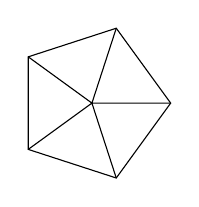
\begin{tikzpicture}
% Define the points of a regular pentagon
\path (0,0) coordinate (origin);
\path (0:1cm) coordinate (P0);
\path (1*72:1cm) coordinate (P1);
\path (2*72:1cm) coordinate (P2);
\path (3*72:1cm) coordinate (P3);
\path (4*72:1cm) coordinate (P4);
% Draw the edges of the pentagon
\draw (P0) -- (P1) -- (P2) -- (P3) -- (P4) -- cycle;
% Add "spokes"
\draw (origin) -- (P0) (origin) -- (P1) (origin) -- (P2)
(origin) -- (P3) (origin) -- (P4);
\end{tikzpicture}
\end{verbatim}





\section{Nodes}

A node is a small part of a picture. When a node is created, you provide a position where the node
should be drawn and a shape. A node of shape circle will be drawn as a |circle|, a node of shape |rectangle|
as a rectangle, and so on. A node may also contain same text, which is why they can used nodes to show text.

Finally, a node can get a name for later reference.



\emphasis{node,shape,draw}
\begin{teXXX}
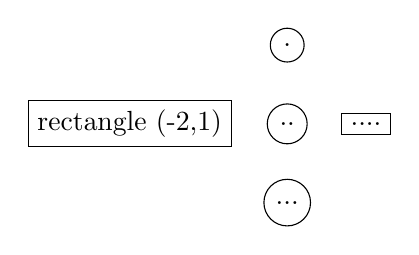
\begin{tikzpicture}
\path ( 0,2) node [shape=circle,draw] {.}
( 0,1) node [shape=circle,draw] {..}
( 0,0) node [shape=circle,draw] {...}
( 1,1) node [shape=rectangle,draw] {....}
(-2,1) node [shape=rectangle,draw] {rectangle (-2,1)};
\end{tikzpicture}
\end{teXXX}
\medskip

\begin{tikzpicture}
\path ( 0,2) node [shape=circle,draw] {1}
( 0,1) node [shape=circle,draw] {\textbf{10}}
( 0,0) node [shape=circle,draw] {\textbf{100}}
( 1,1) node [shape=circle,draw] {\textbf{1000}}
(-2,1) node [shape=circle,draw] {\textbf{10000}};
\end{tikzpicture}

In the above code, this text is empty (because of the
|empty {}|). So, why do we see anything at all at all the nodes? The answer is the draw option for the node operation: It
causes the |shape| around the text" to be drawn. If you have an empty |{}|, PGF still sees the empty space as a character and justs draws around it. The reason is than TikZ automatically adds some space around the text. The amount is set
using the option |inner sep|. So, to increase the size of the nodes. Modifying the example slightly we get.



\begin{tikzpicture}
\path ( 0,2) node [shape=circle,draw] {.}
( 0,1) node [shape=circle,draw] {..}
( 0,0) node [shape=circle,draw] {...}
( 1,1) node [shape=circle,draw] {....}
(-1,1) node [shape=circle,draw] {.....};
\end{tikzpicture}

As you can observe the size of the circle has been adjusted to fit the text that is enclosing it. 
Another way to simply add a node is using the |at| syntax:

\begin{texexample}{The node command}{}
\begin{tikzpicture}
\node at (0,0) [circle, draw] {\textbf{100}};
\node at (1,1) [diamond,draw] {\textbf{100}};
\end{tikzpicture}
\end{texexample}

The \cmd{\node} is an abbreviation of the |\path| node. This is a much shorter syntax than |\path| where one would need to add a lot of redundant move-tos  \seepgfmanual{215}.

If you have many nodes another way of achieving the example outlined above is to use the |\draw| command in comination with node and at.

\begin{texexample}{The node command}{}
\begin{tikzpicture}
\tikz \draw[fill=yellow!80!black]
(0,0) node {first node}
-- (1,1) node[draw, behind path] {second node}
-- (0,2) node[fill=red!20,draw,double,rounded corners] {third node};

\node at (0,0) [circle, draw] {\textbf{100}};
\node at (1,1) [diamond,draw]{\textbf{100}};
\end{tikzpicture}
\end{texexample}

\subsection*{Drawing shapes}

PGF abd \tikzname\ come with a number of predefined shapes:
\begin{itemize}
\item rectangle
\item circle, and
\item coordinate
\end{itemize}


\begin{tikzpicture}
\draw (0,0) circle (1cm);
\draw (0.5,0) circle (0.5cm);
\draw (0,0.5) circle (0.5cm);
\draw (-0.5,0) circle (0.5cm);
\draw (0,-0.5) circle (0.5cm);
\end{tikzpicture}



A circle is specified by providing its center point and the desired radius. The
command:

\medskip

\begin{tikzpicture}
  \draw[step=0.25cm,color=green] (-1,-1) grid (1,1);
  \draw (0,0) circle (1cm);
\end{tikzpicture}
\medskip

\begin{teXXX}
\begin{tikzpicture}
  \draw (x,y) circle (dia);
\end{tikzpicture}
\end{teXXX}



You  can use one |\draw| command to draw multiple circles as shown in \fref{fig:circles}


\begin{tikzpicture} 
 \draw (0,0) 
  circle (1cm)
  circle (0.6cm)
  circle (0.2cm)
 ;
\end{tikzpicture}

\emphasis{circle,begin,end}
\begin{teXXX}
\begin{tikzpicture} 
 \draw (0,0) 
  circle (1cm)
  circle (0.6cm)
  circle (0.2cm)
 ;
\end{tikzpicture}
\end{teXXX}





\begin{center}
\begin{tikzpicture}
\draw (0,0) circle (1cm)
circle (0.6cm)
circle (0.2cm);
\end{tikzpicture}
\captionof{figure}{You can use one draw command to draw multiple circles}
\label{fig:circles}
\end{center}
\captionof{figure}{Drawing multiple circles, using mutiple \texttt{circle} commands}


\subsection{Drawing ellipses}

Ellipses can be drawn in a similar fashion to circles. As an ellipse needs two center points to be specified the command used has the following general form:

\begin{verbatim}
\draw (a,b) ellipse (r1 dim and r2 dim);
\end{verbatim}

We can draw two ellipses as shown in the figure, using the code:
\begin{teX}
\begin{tikzpicture}[scale=0.6]
\draw[color=red] (0,0) ellipse (2cm and 1cm);
\draw[color=red] (0,0) ellipse (1cm and 2cm);
\end{tikzpicture}
\end{teX}

\begin{centering}
\begin{tikzpicture}[scale=0.6]
\draw[color=red] (0,0) ellipse (2cm and 1cm);
\draw[color=red] (0,0) ellipse (1cm and 2cm);
\end{tikzpicture}
\caption[Drawing ellipses]{Use the draw command in combination with ellipse to draw ellipses}
\end{centering}


\begin{teX}
\begin{tikzpicture}
\draw (0,0) ellipse (2cm and 1cm)
ellipse (0.5cm and 1 cm)
ellipse (0.5cm and 0.25cm);
\end{tikzpicture}
\caption{Drawing multiple circles, using mutiple \texttt{draw} commands}
\end{teX}

\section{Drawing more complicated shapes}
we can place a parabola in a rectangle as shown in \fref{fig:parabola}, by using the |rectangle| and the |parabola| options.

\bgroup
\centering

\begin{tikzpicture}
\draw[color=blue] (0,0) rectangle (1,1.5)
(0,0) parabola[color=orange] (1,1.5);
\draw[xshift=1.5cm] (0,0) rectangle (1,1.5)
(0,0) parabola[bend at end] (1,1.5);
\draw[xshift=3cm] (0,0) rectangle (1,1.5)
(0,0) parabola bend (.75,1.75) (1,1.5);
\end{tikzpicture}
\captionof{figure}{Parabolas drawn using the parabola and rectangle options.}
\label{fig:parabola}
\egroup




\emphasis{parabola,rectangle}
\begin{teX}
\begin{tikzpicture}
\draw[color=blue] (0,0) rectangle (1,1.5)
(0,0) parabola[color=orange] (1,1.5);
\draw[xshift=1.5cm] (0,0) rectangle (1,1.5)
(0,0) parabola[bend at end] (1,1.5);
\draw[xshift=3cm] (0,0) rectangle (1,1.5)
(0,0) parabola bend (.75,1.75) (1,1.5);
\end{tikzpicture}
\caption{Parabolas drawn using the parabola command}
\label{fig:parabola}
\end{teX}

\subsection*{The shape library}

\begin{tikzpicture}
\draw [help lines] (0,0) grid (2,2);
\draw [blue, dashed] (1,1) circle(1cm);
\draw [red, dashed] (1,1) circle(.5cm);
\node [star, star point height=.5cm, minimum size=2cm, draw]
at (1,1) {S};
\end{tikzpicture}

\section{Iterations}
One convenient construct provided with TikZ is a |foreach| command sequence

\begin{texexample}{Tikz loops}{tz:ex}
\centering
\begin{tikzpicture}[scale=2, color=bgsexy]
\foreach \i in {1,...,4}
{
  \path (\i,0) coordinate (X\i);
  \fill (X\i) circle (1pt);
}
  \foreach \j in {1,...,3}
{
  \path (\j,1) coordinate (Y\j);
  \fill (Y\j) circle (1pt);
}
\foreach \i in {1,...,4}
{
  \foreach \j in {1,...,3}
  {
     \draw[color=bgsexy] (X\i) -- (Y\j);
  }
}
\end{tikzpicture}
\captionof{figure}{Drawing a bi-partite garph using foreach loops}
\end{texexample}



\section{The pgfplots package}



\subsection{Loading data from files}

Scientific work, especially that associated with research tends to generate
a lot of data. The data would normally come from external applications and stored in files. With |TikZ| one can import the data
by using the word |file|:

\emphasis{addplot,file,x}
\begin{teXXX}
 \addplot file {./raw/wavefunctions/wavefunc\x.dat};
\end{teXXX}

In the example we use a file with a path. The data is saved in
files with the same name but a different ending. We use a |foreach| function to add the ending i.e, the file names are |wavefunc1|, |wavefunc2| and |wavefunc3|. By using external data files and the foreach command it can substantially reduce the amount of text in the macros. This improves debugging and readability.

\begin{texexample}[colback=white]{Loading files}{ex:lfiles}
\centering
\begin{tikzpicture}[scale=0.8]
    \begin{axis}[smooth,
    xlabel=$n$,
    ylabel=$\Theta{j}{n}$]
    \foreach \x in {0,...,2}
    {
        \addplot file {./raw/wavefunctions/wavefunc\x.dat};
    }
    \legend{$j=0$,$j=1$,$j=2$};
    \end{axis}
\end{tikzpicture}
\captionof{figure}{Example plot with data imported from external files, using \texttt{file}}
\end{texexample}


\begin{teXXX}
\begin{tikzpicture}[scale=0.6]
  \begin{axis}[
    xlabel=$n$,
    ylabel=$\Theta{j}{n}$]
    \foreach \x in {0,...,2}
    {
      \addplot file {./raw/wavefunctions/wavefunc\x.dat};
    }
    \legend{$j=0$,$j=1$,$j=2$};
  \end{axis}
\end{tikzpicture}
\end{teXXX}



\section*{Plotting functions}
Functions can be defined for plotting using a variety of methods. They are powerful but generally difficult to remember.



\section{Saving Data to a file}

You can save your data to a file in many ways. One easy way is to use
the \docpkg{filecontents} package. This package extends the LaTeX environment
with the same name, but allows you to overwrite the file {\protect\ctan{filecontents}}.

\begin{teXXX}
\documentclass[justified]{tufte-book}
\usepackage{pgfplots,lipsum,booktabs}
\usepackage{pgfplotstable}
\pgfplotsset{compat=newest}
\usepackage{filecontents*}
\begin{filecontents}{my1.dat}
    Label       value       num
    Integrity     33         4
    Standalone    14         3
    Interface      6         2
    Overall       18         1
\end{filecontents*}
\begin{document}
    your code here ...
\end{document}
\end{teXXX}

It is good practice to keep, such data at the top of your file, although with
the |filecontents| package, they can be inserted anywhere. Sometimes it maybe
easier to have a number of minimal files with the type of charts you using regularly and just update the data on top. In general if the data is entered
by hand rather than generated automatically by software this is a good way
to keep your work tidy.

\newenvironment{Chart}[1][black!70!green]{%
%%  defaults
    \gdef\level##1{Level ##1}
    \def\setchartwidth##1{%
      \def\chartwidth{##1}}%
    \setchartwidth{3.9cm}%
    \def\chartcolor{#1}
    \newcommand\addTitle[2][test]{
    
    
%% For the chart title we set it in a minipage for
%% better control
    \def\charttitle{\minipage{4cm}%
       \footnotesize %
       \centering\textbf{##2}\\##1%
       \endminipage}}%
   \def\xlabel{Completion (\%)}%
%% renders the chart 
    \def\renderChart{%
%%
    \footnotesize%
%%
%%
    \IfFileExists{#1.dat}{Test}{}
   \begin{tikzpicture}
   \begin{axis}[
    xbar, width=\chartwidth,title=\charttitle,
    y=0.5cm, enlarge y limits={true, abs value=0.75},
    xmin=0, xmax=100,enlarge x limits={upper, value=0.25},
    xlabel=\xlabel,
    %ylabel=Label,
    xmajorgrids=true,
    ytick=data,
    yticklabels from table={\dataTable}{Label},
    nodes near coords, nodes near coords align=horizontal
     ]
    \addplot[draw=none, fill=\chartcolor] table [x=value, y=num]
    {\dataTable};
    \end{axis}%
    \end{tikzpicture}}}
{}

\begin{comment}
\begin{figure*}
\centering

\hskip-2cm\begin{Chart}
 \addTitle[Mechanical Systems]{Shangri-la}
 \def\dataTable{SH-mechanical.dat}
 \renderChart
\end{Chart}\hspace{0.3cm}
\begin{Chart}
 \addTitle[FM-200 System]{All areas}
 \def\dataTable{my1.dat}
 \renderChart
\end{Chart}
\begin{Chart}
 \addTitle[Electrical Works]{Merweb}
 \def\dataTable{my6.dat}
 \renderChart
\end{Chart}
\caption{Mechanical Systems Shangrila. Commissioning status}
\end{figure*}


\begin{filecontents*}{my1.dat}
Label     value       num
Integrity         33            4
Standalone      14            3
Interface        6            2
Overall           18            1
\end{filecontents*}

\begin{filecontents*}{SH-mechanical.dat}
Label     value       num
{Fan coil units}       43             8
{Air Handling Units}       13             7 
{CW Pumps}       13             6
{ECU}       11             5
{Pressurization Fans}        15             4
{Smoke Extract Fan}       5             3
{Jet fan}       5             2
{Overall}       12              1
\end{filecontents*}

\begin{filecontents*}{my6.dat}
Label    value         num   other
{Level 7}  50           11   13
L6         90           10   12
L5       80             9    16
L4       90             8    18
L3       70             7    90
L2       80             6    21
L1       70             5    22
\end{filecontents*}

\begin{filecontents*}{carparkventilation.dat}
Label    value         num   other
L5         50           11   13
L4         90           10   12
L3         80           9    16
GR         90           8    18
B1         70           7    90
B2         80           6    21
B3         70           5    22
\end{filecontents*}
%% CO SYSTEM
%% DATA
\begin{filecontents*}{carparkco.dat}
Label    value         num   other
L5         78           7   13
L4         90           6   12
L3         80           5    16
GR         90           4    18
B1         70           3    90
B2         80           2    21
B3         70           1    22
B5         50          {}    {}
\end{filecontents*}

\begin{filecontents*}{carparkco2.dat}
value,   num,   other,
78,       7,   13,
90,       6,   12,
80,       5,    16,
90,       4,    18,
70,       3,    90,
80,       2,    21,
70,       1,    22,
\end{filecontents*}
\end{comment}






















\DocInput{\jobname.dtx}
\backmatter
\printindex
\end{document}
%</driver>
% \fi
% 
%  \CheckSum{0}
%  \CharacterTable
%  {Upper-case    \A\B\C\D\E\F\G\H\I\J\K\L\M\N\O\P\Q\R\S\T\U\V\W\X\Y\Z
%   Lower-case    \a\b\c\d\e\f\g\h\i\j\k\l\m\n\o\p\q\r\s\t\u\v\w\x\y\z
%   Digits        \0\1\2\3\4\5\6\7\8\9
%   Exclamation   \!     Double quote  \"     Hash (number) \#
%   Dollar        \$     Percent       \%     Ampersand     \&
%   Acute accent  \'     Left paren    \(     Right paren   \)
%   Asterisk      \*     Plus          \+     Comma         \,
%   Minus         \-     Point         \.     Solidus       \/
%   Colon         \:     Semicolon     \;     Less than     \<
%   Equals        \=     Greater than  \>     Question mark \?
%   Commercial at \@     Left bracket  \[     Backslash     \\
%   Right bracket \]     Circumflex    \^     Underscore    \_
%   Grave accent  \`     Left brace    \{     Vertical bar  \|
%   Right brace   \}     Tilde         \~}
%
%
%
% \changes{1.0}{2013/01/26}{Converted to DTX file}
%
% \DoNotIndex{\newcommand,\newenvironment}
% \GetFileInfo{phd.dtx}
% 
%  \def\fileversion{v1.0}          
%  \def\filedate{2012/03/06}
% \title{The \textsf{phd} package.
% \thanks{This
%        file (\texttt{phd.dtx}) has version number \fileversion, last revised
%        \filedate.}
% }
% \author{Dr. Yiannis Lazarides \\ \url{yannislaz@gmail.com}}
% \date{\filedate}
%
%
% 
% ^^A\maketitle
% 
% ^^A\frontmatter
%  ^^A\coverpage{./images/hine02.jpg}{Book Design }{Camel Press}{}{}
%  \newpage
% ^^A\secondpage
% \pagestyle{empty}
%
%
% 
%
%
% \pagestyle{headings}
% \raggedbottom
%  \OnlyDescription
%
%  ^^A\StopEventually{\printindex}

% \CodelineNumbered
% \pagestyle{headings}
% 
% 
% ^^A\part{IMPLEMENTATION AND FRIENDS}
% 
% \def\storyi{In this chapter we try and outline the objectives of the package. A lot of effort has been
%              exerted in simplifying the user interface by only defining key value interfaces. Commands and styles can be adjusted without using macros. The package provides a number of pre-defined cover pages, second pages and a method to avoid writing code at the beginning of the document.}
% \chapter{Frontmatter Package Code Implementation Objectives and Strategy}
% 
% \epigraph{
% I was reflecting on the convoluted Java frameworks widely adopted at work. Those hefty frameworks brought coding structures and conventions to large engineering teams; meanwhile, they also sucked the fun of programming like a Pastafarian monster slurping all the tomato sauce on a plate of spaghetti.
%}{\href{http://blog.zmxv.com/2015/07/code-golf-at-google.html}{Zhen Wang}}
%
% \begin{chapterabstract}
%  This chapter describes the implementation part of the code. It has been typeset using the |doc/dtx|. It is about 85\% complete. I am revising it, in tandem with the general ideas described in the \pkg{phd}.
% \end{chapterabstract}
%
% \section{Objectives}
%
% We start by outlining what we are trying to achieve with this package:
%
% \begin{enumerate}
% \item To provide a declarative interface to enable users to change the style
%       of frontmatter, mainmatter and backmatter headings and numbering.
% \item The interface must be able to manupulate properties of headings down to
%       the last detail.
% \item To provide a compatibility mode, where documents wishing to test the package
% can have an easy switch to switch in and out. This is also important for the testing of the package.
% \item To provide a number of templates that cover most of the typical use case.
% \item To provide means for a plug-in architecture for extensions.

% \end{enumerate}
% 
% \section{Terminology}
%
%  \begin{description}
%  \item [document] Any written item, as a book, article, or letter, especially 
%                  of a factual or informative nature.
%  \item [heading] A division of a document or document series. For a normal
%        book headings are chapters, sections etc. However we allow for
%        specifying a more complex document divided into books, volumes
%        parts etc. For example the Bible has Books, chapters and verses,
%        where a legal document might require divisions such as clauses.
%        In general these divisions are numbered. These document divisions
%        are stored in the comma list |phd_book_divisions_clist|.
%  \item [head] A typeset heading, such as chapter head, or section head.
%        This can include a counter, label and title for example, 
%        \emph{Chapter 1 Introduction}.
%  \item [dom] This is a programming interface that provides a structured
%        representation of the document (a tree) and it defines a way
%        that the structure can be accessed. Although \latexe does not
%        offer a standard way to build such a tree (mainly because
%        \tex does not require the marking of paragraphs, it is 
%        useful to think of the document as a tree structure. We also
%        allow for a semi-automated way to build such a tree (with the 
%        exception that paragraphs are not included).
% \item [element] A part of the document tree that can be styled on
%       its own. For example the chapter label, or the section number.
%
% \end{description}
%
% \section{Users}
%  We classify users according to the \LaTeX3 terminology as a) programmers b) template designers
%  and c) authors.
% \subsection{Author}
%  We assume that the author has an exising template which she is using but might want to do
%  some minor modifications, for example use an italic shape for the font of the mark, but an 
%  upright font for the page numbers. 
%
% {\obeylines 
%~~ |\cxset|
%~~~~~|{|
%~~~~~~~~\textit{chapter number color}~~|format          = apa,|
%~~~~~~~~\textit{section title font-size} |font-size   = Large,|
%~~~~~|}|
%}  
%
% We follow the idea of representing the basic elements of documents
% as elements, each one having a parent in order to specify
% the element we need to style as accurate as possible. One can think of
% this approach being congruent with objects in other languages.
% As a matter fact nothing stops us from defining a key value
% interface as shown below.
%
% {\obeylines 
%~~ |\cxset|
%~~~~~|{| 
%~~~~~~~~\textit{header.even.mark.font.size}   = |Large,|
%~~~~~~~~\textit{header.even.mark.font.family} = |serif,|
%~~~~~|}|
%}  
%
% This would pehaps make it easier for the template designer, but I have rejected
% the idea as my aim is to make it easy for the author, who can search the template
% and just enter a couple of new proerty values.
%
% \subsection{Template designer}
% \pagestyle{headings}
% The template designer in the example above would have selected the format style
% from a number of predefined formats (templates) or would have created a style
% called \textit{apa} from an existing template and modified it using declarative
% key style.
%
% \subsection{The programmer}
%
% The programmer in the example above could have created the basic format
% \textit{apa} by using both declarative as well as defining or using existing
% macros. To the programmer we offer an extension mechanism, where the contents
% of a |ps@| command are defined. For example the programmer can define a new
% style using \tikzname, but without having to worry about defining full |ps@|
% and their interface.
%
% \section{Preliminaries}
%
%  Standard file identification. We first announce the package 
%	 and require that it be used with \LaTeX2e. 
% \iffalse
%<*package>
% \fi
%  
%
%    \begin{macrocode}
\NeedsTeXFormat{LaTeX2e}[2017/04/15]%
\ProvidesPackage{phd-frontmatter}[2015/7/13 v1.0 frontmatter management (YL)]%
%    \end{macrocode}
%
% 
% \section{Source2e Interface}
% 
% I am not very fond of mixing expl3 control sequences with source2e commands. Here
% we provide an interface for all these commands we might use. 
% This section can be revisited once expl3 code becomes available.
%
%    \begin{macrocode}
\ExplSyntaxOn
\let\ltxtoday\today
\let\phd_hang_from:nn \@hangfrom
\newif\if@ltxcompat \@ltxcompatfalse
\ExplSyntaxOff
%    \end{macrocode}
% \section{Front matter and backmatter}
%
% These are both provided by the classes but we intent to parameterize them
% so we redefine them.
%
% \subsection{Mainmatter and frontmatter options}
%
% The page numbering options are set by using the source2e defined \docAuxCommand{pagenumbering}.
% 
%    \begin{macrocode}
\ExplSyntaxOn
\newif\if@mainmatter \@mainmattertrue
\cxset{
  frontmatter~numbering/.is~choice,
  frontmatter~numbering/arabic/.code  = \cs_set:Npn \setfrontpagenumbering
                                         {
                                           \pagenumbering{arabic}
                                         },
  frontmatter~numbering/roman/.code   = \cs_set:Npn \setfrontpagenumbering
                                   	     { 
                                           \pagenumbering{roman}
                                         },
  frontmatter~numbering/Roman/.code   = \cs_set:Npn \setfrontpagenumbering 
                                   	     {
                                   	       \pagenumbering{Roman}
                                   	     },
  mainmatter~numbering/.is~choice,
  mainmatter~numbering/arabic/.code  = \cs_set:Npn \setpagenumbering
                                         {
                                           \pagenumbering{arabic}
                                         },
  mainmatter~numbering/roman/.code   = \cs_set:Npn \setpagenumbering
                                   	     { 
                                           \pagenumbering{roman}
                                         },
  mainmatter~numbering/Roman/.code   = \cs_set:Npn \setpagenumbering 
                                   	     {
                                   	       \pagenumbering{Roman}
                                   	     },
                                     	     
  }
\ExplSyntaxOff	
%    \end{macrocode}
% We set the defaults to those of the standard classes.
%    \begin{macrocode}
\cxset{mainmatter numbering = arabic,
       frontmatter numbering = roman}     
%  
%    \end{macrocode}
%
% \begin{docCommand}{frontmatter} {\meta{void}}
%  Handles all the preliminary settings for the frontmatter of a book. It
%  sets \cs{\@mainmatter} to false and handles page openings.   
% \end{docCommand}
%    \begin{macrocode}
\ExplSyntaxOn
\cs_gset:Npn \frontmatter 
  {
    %\cleardoublepage
    \@mainmatterfalse
    \setfrontpagenumbering%
  }
%    \end{macrocode}
% \begin{docCommand}{mainmatter} {\meta{void}}
% Handles all the preliminaries for the main matter of a document.    
% \end{docCommand}
%    \begin{macrocode}
\cs_gset:Npn \mainmatter
  {
    \if@openright\cleardoublepage\else\clearpage\fi
      \@mainmattertrue
     \setpagenumbering
  }
%    \end{macrocode}
% \begin{docCommand}{backmatter}{\meta{void}}
% Analogous to front and mainmatter.
% \end{docCommand}
%    \begin{macrocode}       
\cs_gset:Npn \backmatter
  {
    \if@openright
      \cleardoublepage
    \else
      \clearpage
    \fi
    \@mainmatterfalse
  }
\ExplSyntaxOff      
%    \end{macrocode}      
% 


% \section{Titles, authors, abstracts and the like}
%
% 	We want to have the option to make titles both as normally used in the |book| class
%	but also as used in articles i.e., not to emit a new page after it is invoked.
%	The definition is straight from the article class.
% {@maketitle}
%    This macro takes care of formatting the title information when we
%    have no separate title page.
%
%    We always start a new page, leave some white space and center the
%    information. The title is set in a |\LARGE| font, the author
%    names and the date in a |\large| font. CHECK THIS IF HERE
%    \begin{macrocode}
\def\@maketitle{%
  %\newpage
  \null
  \vskip 2em%
  \begin{center}%
  \let \footnote \thanks
    {\LARGE \@title \par}%
    \vskip 1.5em%
    {\large
      \lineskip .5em%
      \begin{tabular}[t]{c}%
        \@author
      \end{tabular}\par}%
    \vskip 1em%
    {\large \@date}%
  \end{center}%
  \par
  \vskip 1.5em}
  %fi CHECK
%    \end{macrocode}
% 
%
% {maketitle}
%    The macro to generate titles is easily altered in order that it
%    can be used more than once (an article with many titles)\footnote{Definition is straight 	out of the |doc| package and I only added minor tweaks to only start a new page 
%	on demand.}.  In the
%    original, diverse macros were concealed after use with
%    |\relax|. We must cancel anything that may have been put
%    into |\@thanks|, etc., otherwise {\em all\/} titles will
%    carry forward any earlier such setting!
%                 \cs{@makefnmark} and \cs{@makefntext}.
%    \begin{macrocode}
\def\nonewpage{}
\def\maketitle{\par
      \begingroup \def \thefootnote {\fnsymbol {footnote}}%
      \setcounter {footnote}\z@
      \def\@makefnmark{\hbox to\z@{$\m@th^{\@thefnmark}$\hss}}%
      \long\def\@makefntext##1{\parindent 1em\noindent
            \hbox to1.8em{\hss$\m@th^{\@thefnmark}$}##1}%
      \if@twocolumn \twocolumn [\@maketitle ]%
      \else \nonewpage \global \@topnum \z@ \@maketitle \fi
%    \end{macrocode}
%    For special formatting requirements (such as in TUGboat), we use
%    pagestyle |titlepage| for this; this is later defined to be
%    |plain|, unless already defined, as, for example, by
%    |ltugboat.sty|.
%    \begin{macrocode}
       \thispagestyle{titlepage}\@thanks \endgroup
%    \end{macrocode}
%    If the driver file documents many files, we don't want parts of a
%    title of one to propagate to the next, so we have to cancel
%    these, however before we save in another macro for later
%    usage in headers, if required. :
%    \begin{macrocode}
      \setcounter {footnote}\z@
      \gdef\@date{\today}\gdef\@thanks{}%
      \let\doctitle@cx\@title
      \let\docauthor@cx\@author
%
      \gdef\@author{}\gdef\@title{}%
}
%    \end{macrocode}
% 
%
%	As you can see from below, it can now work anywhere. 
% \maketitle
% 
%  Test |\@author| and test |\doctitle@cx| |\docauthor@cx|,
% 
%
%
%% headers and footers
%    \begin{macrocode}
\cxset{
  header style/.store in=\headerstyle@cx,
% general draft rules
  rule /.is choice,
  rule on/.code={\gdef\rulewidth@cx{0.4pt}},
  rule off/.code={\gdef\rulewidth@cx{0pt}},
% headers and footers
  lhead/.code ={\lhead{#1}},
  rhead/.code={\rhead{#1}},
  chead/.code={\chead{#1}},
  lfoot/.code ={\lhead{#1}},
  cfoot/.code={\chead{#1}},
  rfoot/.code={\rhead{#1}},
  headrulewidth/.code={\renewcommand\headrulewidth{#1}},
  footrulewidth/.code={\renewcommand\footrulewidth{#1}},
}
%    \end{macrocode}
% {ps@titlepage}
%	 When a number of articles are concatenated into a
%    journal, for example, it is not usual for the title pages of such
%    documents to be formatted differently.  Therefore, a class
%    such as \textsf{ltugboat} can define this macro in advance.
%    However, if no such definition exists, we use pagestyle
%    \texttt{plain} for title pages.Again the definition is 
%	from the \pkg{doc} package.
%    \begin{macrocode}
\@ifundefined{ps@titlepage}
    {\let\ps@titlepage=\ps@plain}{}
%    \end{macrocode}
% 
%
% \section{Defining Abstracts, summaries, precis, keywords etc}
%
% \subsection{Abstract}
%
% \begin{environment}{abstract}
%
%	This is an interesting environment provided in the standard
%	classes only for articles. However too many publications 
%	require such abstracts in other sections as well so we redefine
%	it here to make it more extensive.
%	
% \begin{docEnvironment}{abstract}{}
%    When we are producing a separate titlepage we also put the
%    abstract on a page of its own. It will be centred vertically on
%    the page.
% \end{docEnvironment}
%
%    Note that this environment is not defined for books.
%         to avoid page break after abstract heading.
%
%    \begin{macrocode}
\def\abstractname{Abstract}
\@ifundefined{abstract}{%
  \newenvironment{abstract}{%
      \titlepage
      \null\vfil
      \@beginparpenalty\@lowpenalty
      \begin{center}%
        \bfseries \abstractname
        \@endparpenalty\@M
      \end{center}}%
     {\par\vfil\null}
%    \end{macrocode}
%
%    When we are not making a separate titlepage --the default for the
%    article document class-- we have to check if we are in twocolumn
%    mode. In that case the abstract is as a |\section*|, otherwise
%    the quotation environment is used to typeset the abstract.
%    \begin{macrocode}
}{}
%    \end{macrocode}
% \end{environment}
%
% \begin{environment}{chapterabstract} This is an identical environment to that
%	provided for abstract and can be used anywhere in the document. 
%    \begin{macrocode}
\def\chapterabstractname{Summary}

\newenvironment{chapterabstract}{%
   \center
     {\bfseries \chapterabstractname\vspace{-.5em}\vspace{\z@}}
   \endcenter\quotation
}{\endquotation}
%    \end{macrocode}
% \end{environment}
%
% \begin{chapterabstract}
%   \lorem
% \end{chapterabstract}
%
% \begin{docCommand} {chapterabstractname} { \meta {void}}  
%  We define a key for the summary or
% 	 or abstract at the top of a chapter. In most cases it is just called a summary.
%  One can use the \cs{chapterabstractname} to change it to another language.
% \end{docCommand}
%     
%    \begin{macrocode} 
\cxset{chapter abstractname/.store in =\chapterabstractname}
\cxset{chapter abstractname= SUMMARY}
%    \end{macrocode}
% 
% 
% \begin{docCommand}{precis} { \marg{text} } Precis is a command to be used for summaries. The same summary 
% can also be used for the toc. 
% \end{docCommand}
%    \begin{macrocode}
\newcommand\precis[1]{%
     \precis@cx{#1}%
     \precistoc@cx{#1}%
     \addvspace{20pt} % check this should be settable
}
%
\def\precis@cx#1{%
\bgroup
\small
\centering
\parbox{.8\textwidth}{#1}
\par\medskip\egroup}

\def\precistoc@cx#1{%
    \addcontentsline{toc}{section}{%
    \bgroup\bgroup#1\egroup\egroup
    %
  }
}
%    \end{macrocode}
%
%    \begin{macrocode}
\newdimen\phdparindent
\setlength{\phdparindent}{12\p@}
\parindent\phdparindent
%    \end{macrocode}
% \begin{docEnvironment}{dedication}{}
%  Koma defines thsi so we provide.
% \end{docEnvironment}
%    \begin{macrocode}
\DeclareDocumentEnvironment{dedication}{}
{\clearemptydoublepage
 \thispagestyle{empty}
 \vspace*{13\baselineskip}
 \large\itshape
\let\\\@centercr\@rightskip\@flushglue \rightskip\@rightskip
\leftskip4cm\parindent\z@\relax
\everypar{\parindent=\phdparindent\let\everypar\empty}}{\clearpage}
%    \end{macrocode}
% 
% 
% \begin{docCommand} {addtocimage@cx} {\meta{} \meta{} \meta{}}
%  Adds an image to the ToC.
% \end{docCommand}
% 
%    \begin{macrocode}
\long\def\addtocimage@cx#1#2#3{%
\tikz[remember picture,overlay] {%
\node[anchor=east,xshift=#1,yshift=#2] at (0,0) {\includegraphics[width=.15\linewidth]{#3}};}%
}
%    \end{macrocode}
%    
%    Adds an image to the ToC.
%    Needs testing for twoside printing. 
%    \begin{macrocode}
\def\addtocimage#1#2#3{%
 \addtocontents{toc}{\protect\addtocimage@cx{#1}{#2}{#3}}%
}
%    \end{macrocode}
% 
%
% \begin{chapterabstract}
%   \lorem
% \end{chapterabstract}
%
% \section{Cover and Second pages}
% 
%	We define author commands for coverpages and
%	second pages. If they have been defined by the
%	author we do nothing, otherwise we provide some
%	defaults as examples.
% \begin{docCommand} {coverpage} {\marg{} \marg{} \marg{} \marg{} \marg{} }
%   Creates a cover page for a document.
% \end{docCommand}
% The design of a cover page---and perhaps a dust cover---is best left to a book
%  designer, here we provide a number of predefined templates for documents
%  that will be primarily viewed on screen.
%
%    \begin{macrocode}
 \ExplSyntaxOn
\cxset
  {
    cover~font-size/.font-size~in = \cover_font_size,
 }

\cs_if_exist:NF \coverpage 
  {
    \DeclareDocumentCommand {\coverpage}  {+O{Y Lazarides} m m m m m }
     {
       \thispagestyle{empty}
       \coverpage_aux:nnnnn {#1} {#2} { #3} {#4} {#5} {#6}
     }

     \cs_new:Npn \coverpage_aux:nnnnn #1 #2 #3 #4 #5 #6
      {
      %\pagecolor{black!80}
      \gdef\coverpageimage{#2}
      \gdef\secondpageimg{#2}
      \vspace*{-3.0cm}
      \parbox[t][0pt]{\textwidth}{%
         \color{black}
         \hbox to \hsize{\hfill\hfill \huge \bfseries\textsf{#1}}
         \vspace*{0.1cm}
         \hskip-3cm\includegraphics[width=\paperwidth]{#2}\par %hine-02
         \vspace*{.8\baselineskip} %3
         \hbox to \hsize{%
         \Huge \hfill\hfill{\MakeUppercase{\bfseries  
         \textsf{\textls{#5}}}}}%
         \vspace*{0.3cm}
         \hbox to \hsize{\Huge \hfill\hfill{\MakeUppercase{\bfseries \textsf{\textls{#6}}}}}
         \vspace*{0.3cm}
         \hbox to \hsize{\huge \hfill\hfill\textsf{\hbox{#3}}}%
         \vspace*{0.3cm}
         \hbox to \hsize{\huge \hfill\hfill\textsf{\hbox{#4}}}%
         
        }
     }
     
  }
  {\thispagestyle{empty} }
  
    
\ExplSyntaxOff
%    \end{macrocode}
% \section{Cover page backgrounds}
% Most cover pages for books can be considered of consisting of two major components:
%  \begin{enumerate}
%    \item A background layer that displays perhaps a full image, patterns or colors
%    \item A foreground layer that consists of \enquote{bands} of text, that
%          describe the book titles, author(s) publishers and the like.
%    \item More layers are also possible. For example in a series of reports,
%          irrespective of any background or foreground we might always wish to display
%          a company logo. To make the templates more flexible this can be placed on
%          its own layer. 
%  \end{enumerate}
%
%  Although possible to have a \tex only solution with boxes, more flexible templates
%  can be developed using \tikzname.
%    \begin{macrocode}
\cxset{doc title/.store in=\doctitle,
       doc authors/.store in=\docauthors,
       coverpage subtitle/.store in = \coverpagesubtitle ,   
       coverpage image/.store in    = \coverpageimage,
       coverpage author/.store in   = \coverpageauthor,
       coverpage authors/.store in  = \coverpageauthors}
       
\cxset{doc title          = DOHA OASIS PROJECT,
       doc authors        = {},
       coverpage subtitle = DESIGN OF ANCILLARY BOOK ELEMENTS,
       coverpage author   = Yannis Lazarides,
       coverpage image    = sebastian}
%
%        
\def\coverpagefullpage{%
\pgfdeclarelayer{logo layer}
\pgfsetlayers{background layer,main,logo layer,foreground layer}
\gdef\secondpageimg{\coverpageimage}%
\thispagestyle{empty} % Suppress headers and footers on the title page
\begin{tikzpicture}[remember picture,overlay]
\node[inner sep=0pt] (background) at (current page.center) {%
  \includegraphics[width=\paperwidth]{\coverpageimage}};
\draw (current page.center) node [yshift=-4cm,fill=theblue!70!white,fill opacity=0.3,text opacity=1,inner sep=1cm]{\Huge\centering\bfseries\sffamily\parbox[c][][t]{\paperwidth}{\color{white}\centering \arial\doctitle \\[15pt] % Book title
{\huge\color{white}  \coverpagesubtitle}\\[20pt] % Subtitle
\coverpageauthor\\
 Nicholas Lazarides\\
 George Lazarides
}%author name
}; % node
%
\begin{pgfonlayer}{logo layer}
\draw (current page.south) node[yshift=1cm,fill=theblue!70!white,text opacity=0.8,
        fill opacity=0.3,inner sep=0.5cm,shape=rectangle,draw]{\parbox[c][][t]{\paperwidth}{\hfill\colorbox{white}{
\includegraphics[width=1cm]{latex3.png}}\hbox to 0.5cm{\space}}};
\end{pgfonlayer}
\end{tikzpicture}
\vfill
\newpage}
%    \end{macrocode}
%
% \begin{docCommand} {secondpage}{\marg{void}}
%   Typesets the second page of a book or report. Parameters need to be set before
%   calling the macro using |\cxset|
% \end{docCommand}
%
%	Although I tried to make it as flexible as possible, it is not a general	command, 
% but rather a command that you will need to redefine to follow house rules. It is included
%	here as an example and to typeset the second page of the documentation.
%
%	\begin{macrocode}
\DeclareDocumentCommand{\SecondPageImageDescription} {m} 
  {
    \long\gdef\secondpageimgdescription{#1}  
  }
  
\SecondPageImageDescription{The cover image shows Jo Bodeon, a back-roper in the mule room at 
    Chace Cotton Mill. Burlington, Vermont. This and other similar images 
    in this book were taken by Lewis W. Hine, in the period between 
    1908-1912. These images as well as social campaigns by many including 
    Hine, helped to formulate America's anti-child labour laws.}
  
\newcommand\secondpage{\clearpage
  \pagecolor{white}
  \null{\Huge\doctitle}\vfill\vfill
  \begin{minipage}[b]{0.9\textwidth}
    \includegraphics[width=3cm]{\secondpageimg}\par
    \raggedright
    \textit{Cover image: }
    \secondpageimgdescription  
  \end{minipage}\par
  \vspace*{\baselineskip}
  \begin{minipage}[b]{0.9\textwidth}
  \RaggedRight
  \setlength{\parskip}{0.5\baselineskip}
    Copyright \copyright 2015  Dr Yiannis Lazarides\par
    Permission is granted to copy, distribute and\slash or modify this document 
    under the terms of the GNU Free Documentation License, version 1.2, with no 
    invariant sections, no front-cover texts, and no back-cover texts.\par
    A copy of the license is included in the appendix.\par
    This document is distributed in the hope that it will be useful, but without 
    any warranty; without even the implied warranty of merchantability or 
    fitness for a particular purpose.
  \end{minipage}
  \vspace*{2\baselineskip}
  \clearpage
}
\cxset{second page texti/.code = \long\def\secondpageimgdescription{\bgroup\parskip1em #1\egroup},
       second page copyright/.code = \def\SecondPageCopyright{#1}}
\cxset{second page texti = {This is some text.}}       
%    \end{macrocode}
% 
%</package>
\endinput





%